\documentclass[final, 12pt, oneside, openright]{class_diss}
\usepackage[utf8]{inputenc}
\usepackage[T1]{fontenc}
\usepackage[spanish, es-tabla]{babel}
\selectlanguage{spanish}
\usepackage{eurosym}
\usepackage{listings}
\usepackage{cancel}
\usepackage{algorithm}
\usepackage{algorithmic}
\usepackage{      amsmath}
\usepackage{     graphicx}
\usepackage{amsxtra}
\usepackage{amssymb}
\usepackage{amsthm}
\usepackage{latexsym}
\usepackage{enumerate}
\usepackage{float}
\usepackage{rotating}
\usepackage[usenames]{color}
\usepackage[table]{xcolor}
\definecolor{  Pink}{rgb}{1.0, 0.5, 0.5}
\definecolor{Maroon}{rgb}{0.8, 0.0, 0.0}
\usepackage[sort&compress]{natbib}
\usepackage[pdftex, plainpages=false, pdfpagelabels]{hyperref}
\usepackage{url}

\hypersetup{
    linktocpage=true,
    colorlinks=true,
    bookmarks=true,
    citecolor=blue,
    urlcolor=blue,https://www.overleaf.com/project/5db83b575ef1b30001f7a93f
    linkcolor=Maroon,
    citebordercolor={1 0 0},
    urlbordercolor={1 0 0},
    linkbordercolor={.7 .8 .8},
    breaklinks=true,
    pdfpagelabels=true,
}

\topmargin      = -0.56in
\textheight     = 8.60in
\textwidth      = 6.46in
\oddsidemargin  = 0.02in

\begin{document}
    \setcounter{page}{-1}
    \newpage


\thispagestyle{empty}


\begin{center}

    \vspace{1cm}


    {\Large Implementación paralela del Automatic Target Detection and Classification Algorithm haciendo uso de la ortogonalización de Gram Schmidt
    para el análisis de imágenes hiperespectrales}\\

    \vspace{1.5cm}

    {\large Andrés Ortiz Loaiza}\\

    \vspace{1.5cm}

    GRADO EN INGENIERÍA DE COMPUTADORES. FACULTAD DE INFORMÁTICA\\
    UNIVERSIDAD COMPLUTENSE DE MADRID \\


    \vspace{0.65cm}
    \rule{2in}{0.5pt}\\
    \vspace{0.85cm}

    
\includegraphics[height=2.5in]{images/ucm/shield2.jpg}

    \vspace{0.5cm}
    Trabajo Fin de Grado en Ingeniería de Computadores

    \vspace{0.5cm}

    Madrid, mayo de 2019\\
    \vspace{3cm}

\end{center}

{\raggedleft
    Directores:\\
    \vspace{ 0.5cm}
    González Calvo, Carlos\\
    Bernabé García, Sergio\\
}
    \pdfbookmark[0]{Cover}{PDFCoverPage}
    \newpage\leavevmode\thispagestyle{empty}\newpage
    \newpage
\thispagestyle{empty}
\begin{center}
{\bf \Huge Agradecimientos}
\end{center}
\vspace{1cm}
\setlength{\baselineskip}{0.8cm}

Gracias a mis profesores por apoyar mis ideas y hacer de este proyecto algo con lo que he podido disfrutar en todo momento.

Por supuesto gracias a mi madre, la persona que siempre ha estado conmigo en todos los momentos buenos y malos de mi vida.
\textit{}
    \phantomsection
    \newpage\leavevmode\thispagestyle{empty}\newpage
    \newpage
    \pagenumbering{roman}
    \setcounter{page}{1}
    \cleardoublepage
    \phantomsection
    \addcontentsline{toc}{chapter}{Índice general}
    \tableofcontents
    \listoffigures
    \listoftables
    \vspace{11cm}
    \newpage
    \cleardoublepage
\begin{center}

{\bf \Huge Resumen}

\end{center}

La observación remota de la Tierra ha sido siempre objeto de interés para el ser humano.
A lo largo de los años los métodos empleados con ese fin han ido evolucionando hasta que, en la actualidad, el análisis de imágenes multiespectrales constituye una línea de
investigación muy activa, en especial para realizar la monitorización y el seguimiento de incendios o prevenir y hacer un seguimiento de desastres naturales, vertidos químicos
u otros tipos de contaminación ambiental.

Las imágenes satelitales en un mundo donde el machine learning y el procesamiento de datos ha avanzado tanto nos abre la posibilidad de construir modelos capaces de reconocer zonas
en las que ha ocurrido un desastre natural y poder actuar en consecuencia.
Con la potencia de cálculo actual podemos conseguir que el procesamiento de los datos sea en tiempo real , por lo que se pueden tomar decisiones para poder minimizar daños, distribuir
equipos de emergencia y optimizar en general todos los recursos que tenemos.

Estos últimos años el campo de la ciencia de datos ha sido capaz de crear modelos precisos en sectores como banca, industria, tecnología.
Pero el círculo solo puede estar completo si podemos
conseguir colocar estos modelos en un entorno en el que se puedan consumir de manera productiva y ser útiles fuera del escenario de desarrollo e investigación.

Mantener toda la infraestructura hardware y software para ejecutar nuestra aplicación es costoso, de la misma manera que contratar a las personas con los conocimientos necesarios
para instalar y configurar todos estos componentes.
El mundo ha evolucionado de manera que ya es no necesario seguir este comportamiento y podemos optar por proveedores que facilitan todos estos componentes
así como el mantenimiento de los mismos, la nube.

En este trabajo de fin de grado se lleva a cabo la optimización en tiempos de inferencia de un modelo de machine learning usado para detectar desastres naturales con OpenVINO a la par que se realiza la puesta a
producción de la aplicación en un entorno cloud de Google, con el objetivo de que nuestro servicio soporte miles de peticiones por minuto.

\vspace{0.8cm}
\begin{center}


{\bf \Large Palabras clave}

\end{center}

Imágenes hiperespectrales, OpenVINO, TensorFlow, Docker, Google Cloud

\vspace{0.3cm}
    \addcontentsline{toc}{chapter}{Resumen}
    \pdfbookmark[0]{Summary}{PDFSummaryPage}
    \newpage
    \begin{center}
{\bf \Huge Abstract}

\end{center}

The remote observation of the Earth has always been an object of interest for the human being.
Over the years, the methods used for this purpose have evolved until, at present, the analysis of hyperspectral images constitutes a very active line of research, especially
to monitor fires or prevent and monitoring natural disasters, chemical discharges or other types of environmental pollution.

Satellite images in a world where machine learning and data processing have advanced so much opens up the possibility of building models capable of recognizing areas where a natural
disaster has occurred and be able to act accordingly.

With the current computing power we can make data processing in real time so we can made decision to minimize damage, distribute emergency teams and optimize all the resources we have.
In recent years the field of data science has been able to create accurate models in sectors such as banking, industry, technology.
But the circle can only be complete if we can manage to place these models in an environment where they can be consumed productively and be useful outside the development and research scenario.

Maintaining all the hardware and software infrastructure to run our application is expensive, in the same way that hiring people with the necessary
knowledge to install and configure all these components.
The world has evolved so that it is no longer necessary to follow this behavior and we can choose suppliers that facilitate all these components as well as their maintenance, the cloud.

In this final degree project, the optimization in inference times of a machine learning model used to detect natural disasters with Openvino is carried out at the same time that the
deploy of the model in a google cloud environment, so that our service supports miles of requests per minute.
%\vspace{1cm}

\vspace{0.8cm}
\begin{center}

{\bf \Large Keywords}

\end{center}

Hyperspectral images, Openvino, Tensorflow, Docker, Google Cloud

\vspace{0.5cm}

\mbox{}

    \addcontentsline{toc}{chapter}{Abstract}
    \pdfbookmark[0]{Abstract}{PDFAbstractPage}
    \vfill
    \newpage
    \pagenumbering{arabic}
    \setcounter{page}{1}

    \cleardoublepage


\chapter{Introducción}
\label{ch:chapter1}


\section{Motivación}

Una imagen hiperespectral es una imagen de gran resolución espectral que se obtiene a través de sensores capaces de obtener cientos o incluso miles de imágenes sobre el mismo área terrestre
pero correspondientes a diferentes canales de longitud de onda.
El conjunto de bandas espectrales no está limitado estrictamente al espectro visible sino que también abarca el infrarrojo y el ultravioleta.

En la actualidad, el uso de imágenes hiperespectrales está aumentando considerablemente debido al lanzamiento de nuevos satélites y el interés en la observación remota de la Tierra,
que tiene utilidad en ámbitos tan diversos como defensa, agricultura de precisión, geología (detección de yacimientos minerales), valoración de impactos ambientales o incluso visión artificial.

\section{Objetivos}

El objetivo principal de este proyecto reside en dos puntos clave.
Por una parte la optimización del tiempo de inferencia en un modelo de machine learning usado para detectar desastres naturales mediante Openvino.
Finalmente el despliegue del modelo en un entorno cloud donde pueda funcionar como un servicio capaz de soportar miles de llamadas concurrentes.
La consecución del objetivo general anteriormente mencionado se lleva a cabo en la
presente memoria abordando una serie de objetivos específicos, los cuales se enumeran a
continuación:
\begin{itemize}
    \item Diseño de módulos individuales en VHDL que sirvan para realizar todas las operaciones que se necesitan para la implementación del algoritmo ATDCA-GS.
    \item Elaboración de una máquina de estados e implementacion del algoritmo usando los modulos individuales.
    \item Análisis y optimización de una implementación paralela previa en OpenCL del algoritmo.
    \item Obtención de resultados y realización de comparativas de rendimiento entre ambos lenguajes de programación.
\end{itemize}

%[CARLOS - INICIO]

%Hablar del objetivo general de realizar la implementación paralela en FPGA del algoritmo Automatic Target Detection and Classification Algorithm haciendo uso de la ortogonalización deGram Schmidt para el análisis de imágenes hiperespectrales.

%La consecución del objetivo general anteriormente mencionado se lleva a cabo en la presente memoria abordando una serie de objetivos específicos, los cuales se enumeran a continuación:

%\begin{itemize}
%\item
%\end{itemize}

%[CARLOS - FIN]


\section{Organización de esta memoria}

Teniendo presentes los anteriores objetivos concretos, se procede a describir la organización del resto de esta memoria, estructurada en una serie de capítulos cuyos contenidos se describen a continuación:

\begin{itemize}
    \item \textbf{Análisis hiperespectral}: se define el concepto de imagen hiperespectral y el modelo lineal de mezcla; se mencionan algunos sensores hiperespectrales (AVIRIS y EO-1 Hyperion) y algunas bibliotecas espectrales (USGS y ASTER); y por último, se presenta la necesidad de paralelización y las plataformas que se pueden utilizar para afrontar el problema de mejora de rendimiento.
    \item \textbf{Tecnología de las FPGAs}: se define de forma breve las tecnologías de las FPGAs.
    \item \textbf{Implementación}: se define el algoritmo ATDCA-GS en serie y se explica la paralelización y optimización que se ha llevado a cabo tanto en VHDL como en OpenCL.
    \item \textbf{Resultados}: se presentan los resultados obtenidos tras la implementación y ejecución del algoritmo en dispositivos FPGAs.
    \item \textbf{Conclusiones y trabajo futuro}: se presentan las principales conclusiones de los aspectos abordados en el trabajo a las que se han llegado y también algunas posibles líneas de trabajo futuro que se pueden desempeñar con relación al presente trabajo.
\end{itemize}

%[CARLOS - INICIO]

%Teniendo presentes los anteriores objetivos concretos, se procede a describir la organización del resto de esta memoria, estructurada en una serie de capítulos cuyos contenidos se describen a continuación:

%\begin{itemize}
%\item
%\end{itemize}

%[CARLOS - FIN]
    %\cleardoublepage
%\newpage
%\thispagestyle{empty}
\mbox{}

\chapter{Análisis hiperespectral}
\label{ch:chapter2}

\section{Imágenes hiperespectrales}

Una imagen hiperespectral (o imagen de gran resolución espectral) es una imagen en la que cada punto (píxel) viene descrito por un conjunto (vector) de valores espectrales que se corresponden con la reflectancia de dicho píxel en diferentes longitudes de onda a estrechas bandas del espectro \cite{biblio:image_clasification}. Cada uno de esos vectores conforman lo que se denomina “firma espectral” \cite{biblio:hyper_analysis, biblio:Tesis_Carlos} del píxel en cuestión, y se obtienen gracias a los sensores hiperespectrales en diversos canales espectrales. El número de bandas que se utilizan suele variar desde las decenas hasta los varios centenares, y el conjunto no está limitado estrictamente al espectro visible sino que también abarca el infrarrojo y el ultravioleta. 

Se puede ver como un caso particular de las imágenes hiperespectrales a las imágenes RGB \cite{biblio:TFM_Pablo_VCA}, las más comunmente utilizadas en el día a día. Ellas están compuestas por tres bandas de color y cada una corresponde a una longitud de onda concreta: rojo, verde y azul, respectivamente. Para componer una imagen RGB a partir de una imagen hiperespectral, se pueden seleccionar esas tres longitudes de onda concretas o las más aproximadas que se encuentren.

Para el estudio de imágenes hiperespectrales se hace uso de la propiedad de reflectancia espectral \cite{biblio:TFG_Esquembri}, que es el porcentaje de energía reflejada sobre la energía incidente como una función de la longitud de onda. La reflectancia es característica de cada material porque varía en función de las distintas longitudes de onda para la mayoría de los materiales dado que la energía puede ser absorbida o reflejada en distintos grados. Por ello, el análisis de estas imágenes sirve también para identificar un material a partir de su firma espectral.

Una imagen hiperespectral puede ser representada como un cubo (denominado “hipercubo” o “cubo hiperespectral”) en el que los ejes X, denominado “líneas” (lines), e Y, denominado “muestras” (samples), se utilizan para mostrar la ubicación espacial de cada píxel de la imagen. El tercer eje Z, denominado “bandas” (bands), se utiliza para mostrar la reflectancia de cada píxel en cada uno de los canales espectrales que haya obtenido el sensor. En la Figura~\ref{fig:cubo hiperespectral} \cite{biblio:TFG_Esquembri} se muestra un ejemplo de cubo hiperespectral, en el que se pueden observar las diferentes bandas de longitudes de onda por separado.

\begin{figure}
  \centering
    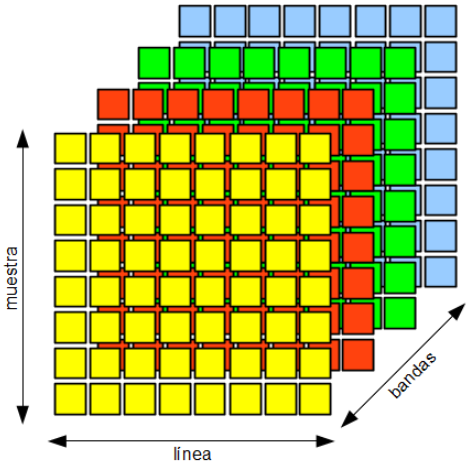
\includegraphics[width=0.5\textwidth]{Imagenes/CuboHiperespectral.png}
  \caption{Ejemplo de cubo hiperespectral.}
  \label{fig:cubo hiperespectral}
\end{figure}

Como se puede observar en la Figura~\ref{fig:pixeles puros y pixeles mezcla} \cite{biblio:TFM_Pablo_VCA}, existen dos tipos de píxeles en función de sus firmas espectrales. Si su firma espectral está constituida por un único tipo de material, el píxel se denomina píxel puro o endmember. Si, por el contrario, está constituida por varios materiales distintos a nivel de subpíxel, el píxel se denomina píxel mezcla. Estos últimos serán los que conformen la mayor parte de la imagen hiperespectral, ya que es muy habitual que cohabiten materiales diferentes en una misma porción de espacio, incluso a nivel microscópico. \cite{biblio:x}.

\begin{figure}
  \centering
    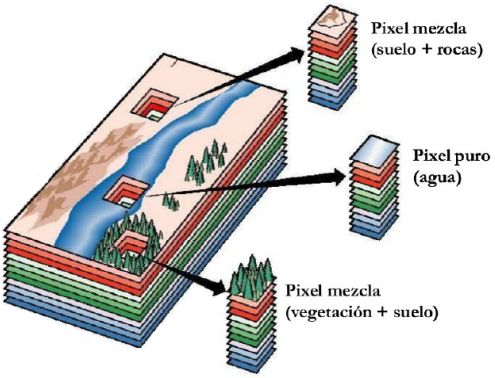
\includegraphics[width=0.6\textwidth]{Imagenes/PixelesPurosPixelesMezcla.png}
  \caption{Ejemplo de píxeles puros y píxeles mezcla.}
  \label{fig:pixeles puros y pixeles mezcla}
\end{figure}

Otro de los aspectos importantes a destacar de este tipo de imágenes es la resolución espectral \cite{biblio:TFM_Pablo_VCA}, que es la separación entre longitudes de onda (a menor separación, mayor resolución espectral) y viene determinada por la tecnología del sensor que se emplea. Cuanto mayor sea la resolución espectral, más información se obtendrá y se podrán esperar mejores resultados en el análisis de las imágenes. Sin embargo, es conveniente tener en cuenta que esta ventaja supone también un aumento considerable del coste computacional.

Las imágenes hiperespectrales surgieron a raíz de las imágenes multiespectrales \cite{landgrebe2003stm}. Este tipo de imágenes se diferencia de las anteriores en que la separación entre bandas es muy grande y la imagen dispone de un número muy pequeño de las mismas (de 4 a 20 aproximadamente). A pesar de basarse en los mismos conceptos, la información proporcionada por las imágenes multiespectrales es mucho más limitada y, por tanto, sus aplicaciones y su método de procesamiento son diferentes \cite{biblio:TFM_Pablo_VCA}.

\section{Sensores hiperespectrales}

El análisis de la Tierra nunca ha dejado de despertar interés o de ser objeto de estudio. Su observación remota se lleva realizando desde hace más de un centenar de años, tradicionalmente empleando cámaras instaladas en globos dirigibles o satélites. No fue hasta el inicio de los años 90 cuando comenzó a surgir la tecnología que serviría para desarrollar los sensores hiperespectrales.

Para obtener las imágenes hiperespectrales, los sensores se basan en la espectroscopia \cite{biblio:TFG_Esquembri}, que es el estudio de la luz emitida o reflejada por los materiales y su variación de energía con la longitud de onda. Esto se consigue empleando unos instrumentos llamados espectrómetros de imágenes, que son capaces de realizar mediciones espectrales de bandas muy próximas entre sí.

El concepto de imagen hiperespectral tuvo su origen en el Jet Propulsion Laboratory\footnote{https://www.jpl.nasa.gov}, una misión comercial de la NASA encargada del desarrollo de instrumentación para la adquisición de imágenes hiperespectrales, esto es, sensores de gran resolución espacial. Un ejemplo de esta instrumentación es el sensor Airborne Visible Infra-Red Imaging Spectrometer (AVIRIS)\footnote{https://aviris.jpl.nasa.gov}.

\subsection{Sensor AVIRIS}

AVIRIS es un sensor óptico creado en 1987 capaz de captar imágenes hiperespectrales de 224 canales espectrales (bandas) con longitudes de onda que varían entre 400 y 2500 nanómetros. Tiene la capacidad de obtener información con un ancho entre bandas (resolución espectral nominal) de 10 nanómetros. Está pensado para ser aerotransportado y analizar zonas del espectro visible e infrarrojo \cite{biblio:result_aviris,biblio:aviris_analysis}.

Este sensor ha realizado tomas de imágenes hiperespectrales en Europa, Estados Unidos, Canadá, Argentina y otras partes de América del Sur mediante el uso de cuatro plataformas de aviones: el jet ER-2, perteneciente al Jet Propulsion Laboratory de la NASA, que vuela a aproximadamente 20 kilómetros sobre el nivel del mar con una velocidad de unos 730 km/h; el turbopropulsor Twin Otter International, desarrollado por la compañía canadiense Havilland Canada, que vuela a 4 kilómetros sobre el nivel del suelo a una velocidad de 130 km/h; el Proteus de Scaled Composites; y el WB-57 de la NASA.

El objetivo principal del proyecto AVIRIS es identificar, medir y monitorizar los componentes de la superficie y la atmósfera terrestre basándose en la absorción molecular y las firmas de dispersión de partículas. Se trata de una investigación centrada principalmente en comprender los procesos relacionados con el medio ambiente y el cambio climático.

%En la Figura~\ref{fig:sensor aviris} se puede observar una imagen de este sensor.

%\begin{figure}
%  \centering
%    \includegraphics{}
%  \caption{Sensor AVIRIS}
%  \label{fig:sensor aviris}
%\end{figure}

\subsection{Sensor EO-1 Hyperion}

Este sensor fue lanzado con éxito en noviembre del año 2000 gracias al programa New Millenium\footnote{http://nmp.nasa.gov} de la NASA. Es capaz de obtener información con una resolución espacial de 30 metros y en 220 bandas espectrales, cubriendo un rango de longitudes de onda de entre 400 y 2500 nanómetros. Cada línea de datos en las imágenes hiperespectrales tomadas está constituida por 256 píxeles.

%En la Figura~\ref{fig:sensor eo-1 hyperion} se puede observar una imagen de este sensor.

%\begin{figure}
%  \centering
%    \includegraphics{}
%  \caption{Sensor EO-1 Hyperion}
%  \label{fig:sensor eo-1 hyperion}
%\end{figure}

\section{Bibliotecas espectrales}

Existen bibliotecas espectrales que facilitan el tratamiento y el análisis de imágenes hiperespectrales. Esto se debe a que contienen una elevada cantidad de datos de reflectancia espectral tanto de materiales naturales como desarrollados por el ser humano. A continuación se nombran algunas de ellas.

\subsection{Biblioteca espectral USGS}

Esta biblioteca fue desarrollada por el laboratorio de espectrometría United States Geological Survey (USGS)\footnote{https://www.usgs.gov}, en Colorado. Contiene información de en torno a 500 reflectancias espectrales, principalmente de minerales, sobre longitudes de onda que varían entre 0.2 y 3.0 micrómetros.

\subsection{Biblioteca espectral ASTER}

Esta biblioteca, impulsada gracias a la NASA, fue desarrollada por el programa Advanced Spaceborne Thermal Emission and Reflectance Radiometer (ASTER)\footnote{http://asterweb.jpl.nasa.gov}. Contiene datos referentes a, aproximadamente, 2000 reflectancias espectrales en un rango de longitudes de onda de entre 0.4 y 14 micrómetros. Dicha información fue recogida a partir de materiales tales como minerales, agua, nieve y otros fabricados por el ser humano, y la tarea se llevó a cabo por el Jet Propulsion Laboratory de la NASA, Johns Hopkins University y United States Geological Survey.

\section{Modelo lineal de mezcla}

Para la realización del desmezclado espectral \cite{biblio:Spectral_unmixing} en el análisis de imágenes hiperespectrales, existen numerosos algoritmos \cite{biblio:varios_alg_desmezclado} y dos modelos principales. El más utilizado actualmente es el modelo lineal de mezcla, que supone que los espectros recogidos en cada pixel mezcla pueden ser representados mediante una combinación lineal de firmas espectrales puras (endmembers). Esta aproximación asume que los componentes que residen a nivel de sub-pixel aparecen separados en el espacio, lo que hace que los fenómenos de absorción y reflexión de la radiación electromagnética incidente puedan ser caracterizados siguiendo un patrón estrictamente lineal y que los efectos producidos por las dispersiones sean mínimos.

\begin{figure}
  \centering
    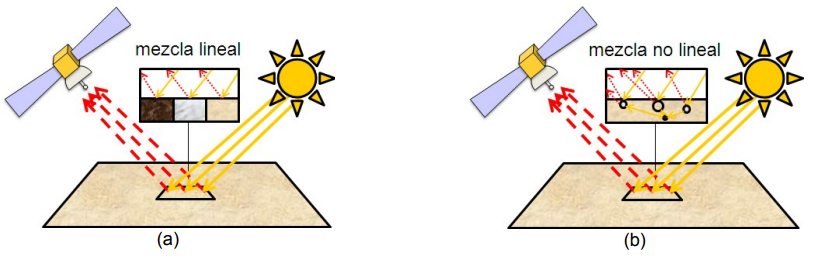
\includegraphics[width=\textwidth]{Imagenes/ComparativaModelosDesmezclado.png}
  \caption{Comparativa entre modelos de desmezclado espectral.}
  \label{fig:comparativa modelos de desmezclado espectral}
\end{figure}

La otra aproximación es el modelo no lineal de mezcla, que tiene en cuenta también aquellos endmembers que se distribuyen al azar a lo largo del campo de visión del sensor, por lo que proporciona una mejor información de la imagen. Sin embargo, para ello requiere información previa acerca de las propiedades físicas de los materiales que conforman la imagen. La Figura~\ref{fig:comparativa modelos de desmezclado espectral} \cite{biblio:TFG_Esquembri} se presenta una comparativa de los dos posibles modelos de desmezclado espectral. Como el modelo no lineal no es aplicable a zonas sobre las que no se posee ninguna información, en este trabajo se opta por utilizar el modelo lineal de mezcla.


Como se puede observar en la Figura~\ref{fig:representacion grafica del modelo lineal de mezcla} \cite{biblio:TFM_Pablo_VCA}, el modelo lineal se puede interpretar gráficamente mediante un espacio bidimensional, utilizando un diagrama de dispersión entre dos bandas de la imagen poco relacionadas entre sí. Todos los puntos de la imagen quedan englobados dentro del área formada por los puntos más extremos, es decir, los elementos espectralmente más puros, que serán los mejores candidatos para ser seleccionados como endmembers.

\begin{figure}
  \centering
    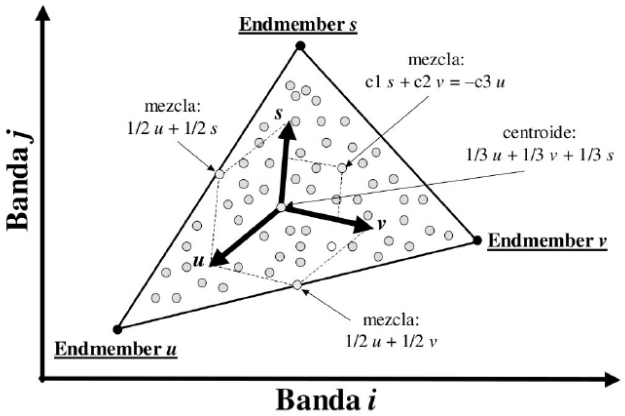
\includegraphics[width=0.7\textwidth]{Imagenes/GraficoModeloLinealDeMezcla.png}
  \caption{Representación gráfica del modelo lineal de mezcla.}
  \label{fig:representacion grafica del modelo lineal de mezcla}
\end{figure}

De esta manera se forman sistemas de coordenadas con origen en el centroide de la nube de puntos y los vectores que van de ese punto a los endmembers. Así, cualquier punto de la imagen puede expresarse como combinación lineal de los endmembers entre los que se encuentre. El paso clave a la hora de aplicar el modelo lineal de mezcla consiste, pues, en identificar de forma correcta los elementos extremos de la nube de puntos N-dimensional. Para ello existen numerosos algoritmos de extracción de endmembers, como el Automatic Target Detection and Classification Algorthm empleado en el presente trabajo.

Se ha optado por el algoritmo ATDCA-GS ya que en trabajos previos se ha hecho uso de arquitecturas CPUs o GPUs y el rendimiento obtenido ha sido suficiente para poder realizar un procesamiento en tiempo real, además de que puede mejorar la precisión si se compara con el algoritmo ATDCA-OSP. También se trata de un algoritmo sencillo pero al mismo tiempo bastante robusto, con operaciones no muy costosas en términos computacionales. Por ejemplo, si de nuevo lo comparamos con el algoritmo ATDCA-OSP, la operación de calcular la inversa de una matriz para obtener las proyecciones ortogonales se sustituyen por la optimización del método de Gram Schmidt, de manera que la complejidad y el tiempo de ejecución se reducen considerablemente.

\section{Necesidad de paralelización}

La mayoría de las técnicas de análisis hiperespectral desarrolladas hasta la fecha, incluyendo la utilizada en este trabajo, tienen en cuenta que gran parte de los píxeles obtenidos por el sensor (píxeles mezcla) vienen dados por la contribución de diversos materiales que residen a nivel de sub-píxel. Por ello, son necesarios diseños capaces de modelar este fenómeno de manera adecuada, lo cual supone un coste computacional considerablemente alto.

Además, la elevada cantidad de datos que se obtienen de cada imagen hiperespectral (las bandas puede ser de cientos o incluso miles de longitudes de onda diferentes) no sólo dificulta la manera en que estos deben ser almacenados y procesados en un ordenador determinado, sino que añade la complicación de que esta información debe ser enviada previamente por el satélite que se ha encargado de la toma de las imágenes.

Existen posibles soluciones al problema de la alta dimensionalidad de los datos \cite{biblio:reducir_dimensiones}. Por un lado, se podría realizar una compresión de datos con pérdidas (mayor compresión pero menos información) o sin pérdidas (menor compresión pero manteniendo la información) \cite{biblio:compresion}. Por otro lado, se podría recoger de manera selectiva determinadas bandas espectrales en base a los materiales sobre los que se requiera información, por ejemplo, minerales y rocas en zonas mineras; o vegetación y agua en zonas de selva o bosque.

Debido a lo anterior, unido a que muchas aplicaciones de observación remota requieren capacidades de procesamiento en tiempo real, se hace imprescindible el uso de arquitecturas paralelas para el procesamiento eficiente y rápido de este tipo de imágenes. Esta tarea resulta relativamente sencilla puesto que al analizar las imágenes se hace uso de operaciones matriciales cuyo carácter repetitivo las hace altamente susceptibles de ser implementadas en arquitecturas paralelas.

En la actualidad, existen múltiples alternativas hardware para la computación paralela: procesadores multi-cores, GPUs o hardware dedicado como los Circuitos Integrados de Aplicación Específica (ASICs) o las FPGAs. De todas ellas, estas últimas presentan una opción eficiente en cuanto a rendimiento haciendo que los tiempos de respuesta sean reducidos y que el algoritmo se ejecute de manera más eficiente. También utiliza una cantidad menor de recursos, por lo que es una de las pocas alternativas que se pueden adaptar en un sensor para poder realizar un procesamiento a bordo.
    \cleardoublepage
%\newpage
%\thispagestyle{empty}
\mbox{}

\chapter{Tecnología de las FPGAs}
\label{ch:chapter3}

Las FPGAs (Field Programmable Gate Arrays) \cite{biblio:Tesis_Carlos} son dispositivos hardware programables y reconfigurables de bajo consumo que ofrecen un gran equilibrio entre flexibilidad y eficiencia, motivos por los cuales han sido elegidas para la implementación del algoritmo en este trabajo. Consisten en una matriz de bloques lógicos o LB (Logic Blocks) y una red de interconexión que pueden ser configurados haciendo uso de dispositivos anti–fuse \cite{biblio:Tesis_Carlos} o mediante un mapa de bits (bitstream) \cite{biblio:bitstream} según la funcionalidad que se requiera.

Los LBs interconectados mediante esa red contienen típicamente uno o varios circuitos combinacionales programables Look-Up Table (LUT), uno o varios biestables, lógica adicional y las celdas de memoria SRAM requeridas para la configuración de todos los elementos. Las tareas de entrada/salida se realizan en la periferia del dispositivo mediante LBs o mediante bloques específicos denominados Input–Output–Blocks (IOBs). La figura~\ref{fig:modelo generico fpga} \cite{biblio:Tesis_Carlos} muestra la estructura interna simplificada de una FPGA.

\begin{figure}
  \centering
    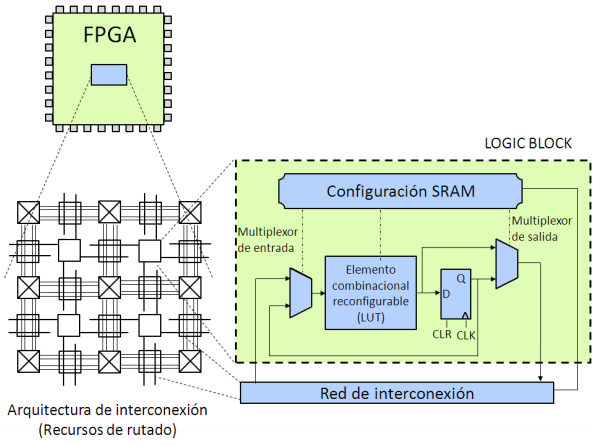
\includegraphics[width=0.8\textwidth]{Imagenes/ModeloGenericoFPGA.png}
  \caption{Modelo genérico de una FPGA.}
  \label{fig:modelo generico fpga}
\end{figure}

%[CarlosIni]Hay que contar que las FPGAs actuales tienen recursos hetereogéneos como memoerias, DSPs y hasta procesadores.[CarlosFin]

Actualmente, se integran también de forma habitual recursos heterogéneos como bloques de memoria RAM dedicada \cite{biblio:ram_dedicada}, multiplicadores, interfaces para periféricos, DSPs (Digital Signal Processor) e incluso microprocesadores. Con la integración de estos elementos arquitectónicos en FPGAs que disponen de una sección de lógica programable por el usuario surge el concepto de Arquitecturas Híbridas \cite{biblio:bitstream}.

El diseño con FPGAs se lleva a cabo mediante un proceso automático conocido como síntesis de alto nivel. Los algoritmos o las tareas deben ser descritos en un lenguaje de alto nivel que esté directamente relacionado con elementos hardware para su fácil traducción a un circuito. En los últimos años se ha utilizado mayormente los lenguajes de descripción hardware (HDL, Hardware Description Language), entre los que destacan Verilog y VHDL.

El primer paso para sintetizar una tarea a hardware es describir el algoritmo en alguno de los HDLs disponibles (por ejemplo, VHDL). El siguiente paso es determinar qué tipo de bloques hardware son necesarios y cómo están conectados entre sí para después, en el tercer paso, asignar bloques básicos configurables concretos de la FPGA (CLBs) y el rutado de señales entre ellos. En el cuarto paso del proceso se obtiene el mapa de bits de configuración necesario para que los LBs utilizados en el diseño del circuito realicen cada uno la funcionalidad necesaria. Por último, es necesario escribir dicho mapa de bits en la memoria de configuración del dispositivo.

Las ventajas que presentan las FPGAs son el aumento de la velocidad de procesamiento \cite{biblio:TFG_Esquembri}, ya que, además de presentar la posibilidad real de paralelización, una ejecución hardware es habitualmente más rápida que el código software; la reducción del consumo, ya que se pueden aplicar técnicas para evitar el consumo innecesario; flexibilidad \cite{biblio:embedded}, ya que existe la posibilidad de reconfigurar los elementos básicos; y el coste reducido debido al aumento de su popularidad y a los avances en la fabricación de su tecnología.

Por otra parte, existen dos aspectos importantes a tener en cuenta \cite{biblio:TFG_Esquembri}: uno es el rutado de las señales, ya que el obtenido tras la compilación no suele ser el más eficiente y suele ser necesaria una revisión manual por parte del diseñador. La solución por la que se opta para mejorar este aspecto es el diseño 3D \cite{biblio:diseno3d}. El otro aspecto es el elevado tiempo de configuración debido al gran tamaño que suele tener el mapa de bits necesario. Ya se están dirigiendo numerosos esfuerzos en nuevas arquitecturas o tecnologías que permitan paliar este efecto.

%\newpage
%\thispagestyle{empty}
%\mbox{}
    \cleardoublepage
\mbox{}

\chapter{Implementación}
\label{ch:chapter4}

%\section{Paradigma de programación paralela OpenCL}

\section{Algoritmo ATDCA-GS en serie}

Anteriormente se ha presentado el problema que supone la existencia de firmas espectrales mixtas en varios píxeles de las imágenes hiperespectrales. La primera etapa del desmezclado espectral permite obtener los endmembers o firmas espectrales puras presentes, lo cual es necesario en la segunda etapa para el procesamiento posterior de la imagen y para la obtención de la presencia cuantitativa de dichos endmembers en cada pixel \cite{biblio:Spectral_unmixing_via}.

Como alternativa a la extracción de endmembers en la primera etapa, existen algoritmos orientados a la detección de targets, como es el caso del algoritmo ATDCA-GS implementado en este trabajo. Los targets son objetivos con características espectrales muy diferentes entre sí. Así, el conjunto de targets de una imagen ofrece una colección de firmas espectrales representativa de los distintos elementos que se pueden encontrar en la imagen.

Se puede realizar una similitud entre targets y endmembers puesto que estos últimos también representan una colección de firmas espectrales muy diferenciadas; sin embargo, es preciso destacar que los endmembers están asociados a firmas espectrales estrictamente puras mientras que los targets son una muestra representativa de los elementos presentes en la imagen.

Generalmente los algoritmos de detección de targets suelen funcionar de manera iterativa, obteniendo cada target en una iteración del algoritmo y, como resultado tras la ejecución, el conjunto de targets detectados. En algoritmos como el ATDCA también se requiere al comienzo una inicialización del conjunto de targets, siendo el píxel más brillante de la imagen (el de mayor intensidad) el más utilizado como primer target. Pese a no ser la única alternativa viable, se ha demostrado experimentalmente que dicho píxel siempre figura en el conjunto de píxeles de la solución \cite{biblio:y}, por lo que supone una elección correcta.

El algoritmo ATDCA usa el concepto de proyección ortogonal de un subespacio para hallar los targets en la imagen. Después de inicializarlo con el pixel más brillante, el siguiente objetivo será aquel con el valor de proyección más alto y será incluido en el subespacio para repetir el proceso tantas veces como targets se quieran detectar. Para optimizar el rendimiento del algoritmo, se ha empleado la ortogonalización de Gram Schmidt, que permite sustituir operaciones complejas, como invertir una matriz, por operaciones más simples y menos costosas en computación. En el Algoritmo~\ref{algoritmo atdca-gs vhdl} se muestra una implementación de este algoritmo en pseudocódigo.

\begin{algorithm}\small
\caption{Algoritmo ATDCA-GS}
\begin{algorithmic}[1]
\label{algoritmo atdca-gs vhdl}
%\STATE H $\leftarrow{}$ imagen hiperespectral de entrada
%\STATE nb $\leftarrow{}$ número de bandas de la imagen
%\STATE r $\leftarrow{}$ número de píxeles de la imagen
%\STATE w $\leftarrow{}$ un array de 1's en punto flotante de 32 bits
%\STATE t $\leftarrow{}$ número de targets a calcular
%\STATE P $\leftarrow{}$ array de posiciones de los targets en la imagen
%\STATE
\STATE \# Cálculo del píxel más brillante
\STATE max = 0
\FOR{$i=0 \text{ to } r-1$}
    \STATE brillo = H[:,i] * H[:,i]$^{T}$
    \IF{$brillo > max$}
        \STATE max = brillo
        \STATE pos = i
    \ENDIF
\ENDFOR
\STATE U[:,0] = H[:,pos]
\STATE P[0] = pos
\STATE
\STATE \# Cálculo del resto de targets
\FOR{$i=0 \text{ to } t-2$}
    \STATE UC = U[:,0..i]
    \IF{$i==0$}
        \STATE f[:,0] = $\sum_{k=0}^{nb-1}UC[k,0]$ / UC[nb,0]
        \STATE u[:,0] = UC[:,0]
        \STATE c2[0] = $\sum_{k=0}^{nb}u[k,0]$ / (u[:,0]$^{T}$ * u[:,0])
    \ELSE
        \STATE c1 = (u[:,0..(i-1)]$^{T}$ * UC[:,i]) / (u[:,0..(i-1)] * u[:,0..(i-1)])
        \STATE u[:, i] = UC[:,i] - $\sum_{k=0}^{i-1}(c1 * u[:,k])$
        \STATE c2 = $\sum_{k}(u[:,k])$ / (u[:,i]$^{T}$ * u[:,i])
        \STATE f[:,i] = w - $\sum_{k=0}^{i}(c2 * u[:,k])$
    \ENDIF
    \STATE
    \STATE max = 0
    \STATE \# Cálculo del píxel más diferente
    \FOR{$j=0 \text{ to } r-1$}
        \STATE result = f[:,i] * H[:,j]
        \STATE val = result$^{T}$ * result
        \IF{$val > max$}
            \STATE max = val
            \STATE pos = j
        \ENDIF
    \ENDFOR
    \STATE U[:,i+1] = H[:,pos]
    \STATE P[i+1] = pos
\ENDFOR
\end{algorithmic}
\end{algorithm}

\section{Paralelización y optimización del algoritmo ATDCA-GS usando VHDL}

Para la implementación en VHDL, se ha construido el módulo descrito gráficamente en la Figura~\ref{fig:modulo atdca-gs vhdl}. A continuación se muestra una secuencia de pasos del funcionamiento del algoritmo en VHDL y en las siguientes subsecciones se mostrarán los sub-componentes que se han empleado y una breve descripción de los mismos.

Usando como referencia el Algoritmo~\ref{algoritmo atdca-gs vhdl}, el código VHDL comienza utilizando los módulos Producto Escalar (línea 4) y Píxel Más Distinto (líneas 5 a 8) para calcular el píxel más brillante, esto es, el primer target de la solución.

Acto seguido se procede a calcular el segundo target empleando los módulos Producto Escalar Auxiliar en modo sólo suma y Divisor en la línea 17; y los módulos Producto Escalar Auxiliar en modo sólo suma, Producto Escalar y Divisor en la línea 19. Después de realizar estos cálculos, procede a calcular con ellos el píxel más distinto utilizando los módulos Producto Escalar Auxiliar en modo sólo multiplicación (línea 30) y Píxel Más Distinto (líneas 31 a 35).

Una vez obtenidos los dos primeros targets, el resto se calcularán haciendo uso de los módulos Producto Escalar, Producto Escalar Auxiliar en modo producto escalar y Divisor (línea 21); los módulos Array Resta Con Acumulación y Producto Escalar Auxiliar en modo sólo multiplicación (línea 22); los módulos Producto Escalar Aux en modo sólo suma, Registro Auxiliar, Producto Escalar y Divisor (línea 23); y los módulos Array Resta Con Acumulación y Producto Escalar Auxiliar en modo sólo multiplicación (línea 24). Después de realizar estos cálculos, se procede a calcular con ellos el píxel más distinto de la misma manera que ocurría para calcular el segundo target.

%[CARLOS - INICIO] Una vez que el algoritmo en serie esté descrito y antes de describir los módulos, pondría una especie de secuencia de pasos de cómo funciona el algoritmo en VHDL (así sirve para darle significado a los módulos aunque aun no se haya descrito su arquitectura)[CARLOS - FIN]

\begin{figure}
  \centering
    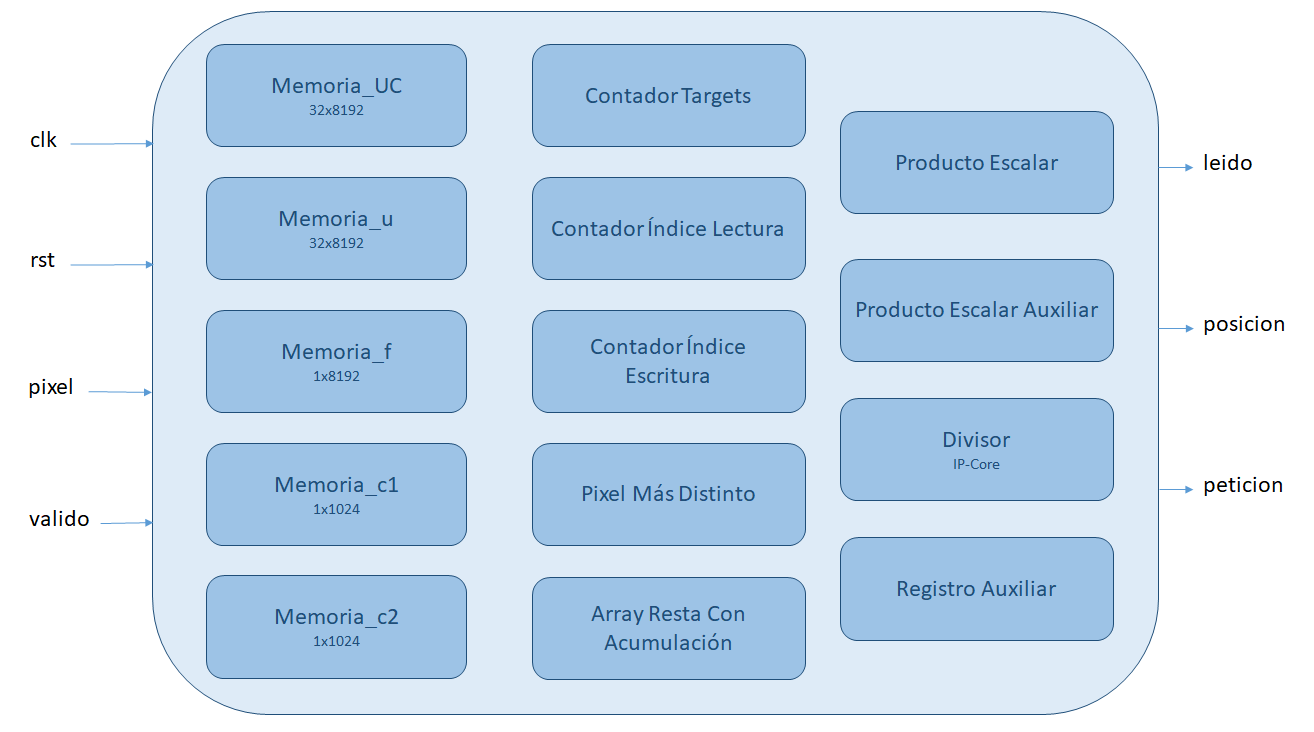
\includegraphics[width=1\textwidth]{Imagenes/DiagramaModuloATDCA-GS.png}
  \caption{Representación gráfica del módulo ATDCA-GS implementado en VHDL.}
  \label{fig:modulo atdca-gs vhdl}
\end{figure}

\subsection{IP-Cores}

Un IP-Core es un componente básico ya implementado que se encuentra incorporado en la herramienta IP-Core Generator dentro del software de desarrollo Xilinx ISE. La principal ventaja que presentan radica en que han sido específicamente diseñados para ser utilizados en dicha herramienta y, por consiguiente, ya han sido completamente optimizados. Se emplean durante el diseño de algoritmos para facilitar enormemente la construcción de operaciones matemáticas complejas y bloques de memoria.

A lo largo de la programación en VHDL del algoritmo ATDCA-GS se han utilizado algunos de los siguientes bloques IP-Core, cuya configuración y descripción se mostrará a continuación.

\subsubsection{Operadores de punto flotante}

Estos componentes hacen uso de una señal de entrada llamada operation$\_$nd, que indica al módulo que los operadores ya están disponibles y debe comenzar a realizar los cálculos. También hacen uso de una señal de salida llamada rdy (ready), que indica que el componente ha terminado de operar y el resultado está ya disponible.

Estos módulos se han utilizado para trabajar con números en punto flotante de precisión simple (32 bits) y están segmentadas, es decir, admiten la entrada de una secuencia consecutiva de datos. Tras una latencia inicial, se irá produciendo un resultado en cada ciclo y en el mismo orden que llevaba la secuencia de entrada.

\begin{itemize}
    \item Restador (restadorPF32Bits.xco)
        \begin{itemize}
            \item IP-core: Floating-point.
            \item Functions: Add/Substract (Substract).
            \item Floating-point precision of A/B inputs: single (32 bits).
            \item Architecture optimizations: Low latency.
            \item Family optimizations: No usage (= Logic only).
            \item Latency: 0.
            \item Cycles per operation: 1.
        \end{itemize}
    \item Divisor (div$\_$escalar$\_$PF32Bits.xco)
        \begin{itemize}
            \item IP-core: Floating-point.
            \item Functions: Divide.
            \item Floating-point precision of A/B inputs: single (32 bits).
            \item Architecture optimizations: High speed.
            \item Family optimizations: No usage (= Logic only).
            \item Latency: Use maximum latency (28).
            \item Cycles per operation: 1.
        \end{itemize}
    \item Comparador (cmp$\_$mayor.xco)
        \begin{itemize}
            \item IP-core: Floating-point.
            \item Functions: Compare (Greater than).
            \item Floating-point precision of A/B inputs: single (32 bits).
            \item Architecture optimizations: High speed.
            \item Family optimizations: No usage (= Logic only).
            \item Latency: 0.
            \item Cycles per operation: 1.
        \end{itemize}
    \item Sumador (sumadorPF32Bits.xco)
        \begin{itemize}
            \item IP-core: Floating-point.
            \item Functions: Add/Substract (Add).
            \item Floating-point precision of A/B inputs: single (32 bits).
            \item Architecture optimizations: High speed.
            \item Family optimizations: Full usage (= 2 x DSP48E).
            \item Latency: 2.
            \item Cycles per operation: 1.
        \end{itemize}
    \item Multiplicador (multiplicadorPF32Bits.xco)
        \begin{itemize}
            \item IP-core: Floating-point.
            \item Functions: Multiply.
            \item Floating-point precision of A/B inputs: single (32 bits).
            \item Architecture optimizations: High speed.
            \item Family optimizations: Full usage (= 2 x DSP48E).
            \item Latency: 1.
            \item Cycles per operation: 1.
        \end{itemize}
\end{itemize}

\subsubsection{Bloques de memoria}

Estos componentes son bloques de memoria que permiten seleccionar un tamaño y unas características concretas tales como los tipos de puertos o la prioridad de lectura o escritura. De esta manera se han podido diseñar bloques de memoria específicos según las necesidades del algoritmo. En concreto, se han utilizado 4 bloques de memoria distintos:

\begin{itemize}
    \item Memoria 2x4096 2 True Dual Port (memoria2x4096$\_$WRITE$\_$FIRST.xco)
        \begin{itemize}
            \item IP-core: Block Memory Generator.
            \item Memory type: True Dual Port RAM.
            \item Port A - Read/Write width: 4096.
            \item Port A - Read/Write depth: 2.
            \item Port A - Operating mode: Write first.
            \item Port B - Read/Write width: 4096.
            \item Port B - Read/Write depth: 2.
            \item Port B - Operating mode: Write first.
        \end{itemize}
    \item Memoria 1x1024 (mem1x1024.xco)
        \begin{itemize}
            \item IP-core: Block Memory Generator.
            \item Memory type: Simple Dual Port RAM.
            \item Common clock.
            \item Port A - Write width: 1024.
            \item Port A - Write depth: 2.
            \item Port A - Operating mode: Read first.
            \item Port B - Read width: 1024.
            \item Port B - Read depth: 2.
            \item Port B - Operating mode: Read first.
            \item Fill Remaining Memory Locations: 0 (Hex).
        \end{itemize}
    \item Memoria 2x4096 Simple Dual Port (memoria2x4096.xco)
        \begin{itemize}
            \item IP-core: Block Memory Generator.
            \item Memory type: Simple Dual Port RAM.
            \item Port A - Write width: 4096.
            \item Port A - Write depth: 2.
            \item Port A - Operating mode: Write first.
            \item Port B - Read width: 4096.
            \item Port B - Read depth: 2.
            \item Port B - Operating mode: Write first.
        \end{itemize}
    \item Memoria 32x4096 (memoria.xco)
        \begin{itemize}
            \item IP-core: Block Memory Generator.
            \item Memory type: Simple Dual Port RAM.
            \item Port A - Write width: 4096.
            \item Port A - Write depth: 32.
            \item Port A - Operating mode: Write first.
            \item Port B - Read width: 4096.
            \item Port B - Read depth: 32.
            \item Port B - Operating mode: Write first.
            \item Fill Remaining Memory Locations: 0 (Hex).
        \end{itemize}
\end{itemize}

\subsection{Módulos VHDL}

A continuación se definen los módulos VHDL que se han implementado para este trabajo.

\subsubsection{Memoria 32x8192 (mem$\_$32x8192.vhd)}

\begin{itemize}
    \item DESCRIPCIÓN
        \begin{itemize}
            \item Memoria de doble puerto simple, es decir, permite realizar una escritura (puerto A) y una lectura (puerto B) simultáneamente. Combina dos memorias de 32x4096 para generar una de 32x8192. Tiene una política de Write First, lo que significa que la lectura garantiza que el dato leído esté siempre actualizado. Está estructurada para almacenar datos de 8192 bits, que sirven para representar un máximo de 256 bandas de 32 bits cada una. Esos 32 bits son los necesarios para representar un número en punto flotante de precisión simple. Tiene 32 filas, una por cada target que se vaya a detectar y almacenar durante la ejecución del algoritmo. No se esperan más de 32 como máximo.
        \end{itemize}
    \item INPUT
        \begin{itemize}
            \item clka: señal de reloj del puerto A.
            \item wea: señal Write Enable que indica si se debe realizar una escritura (1) o no (0).
            \item addra: señal de 5 bits que indica la dirección de memoria sobre la que va a trabajar el puerto A.
            \item dina: señal de 8192 bits que indica el dato que entra por el puerto A.
            \item clkb: señal de reloj del puerto B.
            \item addrb: señal de 5 bits que indica la dirección de memoria sobre la que va a trabajar el puerto B.
        \end{itemize}
    \item OUTPUT
        \begin{itemize}
            \item doutb: señal de 8192 bits que indica el dato que sale por el puerto B.
        \end{itemize}
    \item UTILIZADO EN
        \begin{itemize}
            \item Memoria UC.
            \item Memoria u.
        \end{itemize}
\end{itemize}

\subsubsection{Memoria 1x8192 (mem$\_$1x8192.vhd)}

\begin{itemize}
    \item DESCRIPCIÓN
        \begin{itemize}
            \item Memoria de doble puerto simple, es decir, permite realizar una escritura (puerto A) y una lectura (puerto B) simultáneamente. Combina dos memorias de 2x4096 para generar una de 1x8192. Tiene una política de Write First, lo que significa que la lectura garantiza que el dato leído esté siempre actualizado. Está estructurada para almacenar datos de 8192 bits, que sirven para representar un máximo de 256 bandas de 32 bits cada una. Esos 32 bits son los necesarios para representar un número en punto flotante de precisión simple. Tiene 2 filas pero sólo se utilizará una. Esta fila almacenará la proyección calculada en cada iteración del algoritmo.
        \end{itemize}
    \item INPUT
        \begin{itemize}
            \item clka: señal de reloj del puerto A.
            \item wea: señal Write Enable que indica si se debe realizar una escritura (1) o no (0).
            \item addra: señal de 1 bit que indica la dirección de memoria sobre la que va a trabajar el puerto A.
            \item dina: señal de 8192 bits que indica el dato que entra por el puerto A.
            \item clkb: señal de reloj del puerto B.
            \item addrb: señal de 1 bit que indica la dirección de memoria sobre la que va a trabajar el puerto B.
        \end{itemize}
    \item OUTPUT
        \begin{itemize}
            \item doutb: señal de 8192 bits que indica el dato que sale por el puerto B.
        \end{itemize}
    \item UTILIZADO EN
        \begin{itemize}
            \item Memoria f.
        \end{itemize}
\end{itemize}

\subsubsection{Memoria c (memoriac.vhd)}

\begin{itemize}
    \item DESCRIPCIÓN
        \begin{itemize}
            \item Memoria de doble puerto simple, es decir, permite realizar una escritura (puerto A) y una lectura (puerto B) simultáneamente. Tiene una política de Read First, lo que significa que la lectura garantiza que el dato leído no sea el sobreescrito por la escritura. Está estructurada para almacenar datos de 32 bits agrupados dentro de una única fila de 1024 bits. Por tanto, se representan 32 números (número máximo de targets) de 32 bits cada uno. Esos 32 bits son los necesarios para representar un número en punto flotante de precisión simple. Tiene 2 filas pero sólo se utilizará una. Esta fila almacenará el cálculo generado para el target que corresponda en cada momento en función de la iteración del algoritmo en la que nos encontremos.
        \end{itemize}
    \item INPUT
        \begin{itemize}
            \item clk: señal de reloj del puerto A.
            \item wea: señal Write Enable que indica si se debe realizar una escritura (1) o no (0).
            \item pos: señal de 5 bits que indica qué 32 bits de la única fila de la memoria deben ser modificados en la escritura.
            \item dina: señal de 32 bits que indica el dato que entra por el puerto A.
        \end{itemize}
    \item OUTPUT
        \begin{itemize}
            \item doutb: señal de 1024 bits que indica el dato que sale por el puerto B.
        \end{itemize}
    \item UTILIZADO EN
        \begin{itemize}
            \item Memoria c1.
            \item Memoria c2.
        \end{itemize}
\end{itemize}

\subsubsection{Contador (contador$\_$rst.vhd)}

\begin{itemize}
    \item DESCRIPCIÓN
        \begin{itemize}
            \item Contador módulo n comenzando desde 0. En cada flanco de reloj, si la señal count$\_$up está a 1, se suma 1 al valor actual del contador. Si está a 0, no se produce ningún cambio. Por la señal dout sale el valor por el que vaya la cuenta del contador en cada flanco de reloj. Las señales rst y rst$\_$sync, si están a 1, reinician el contador haciendo que la cuenta comience de nuevo en 0.
        \end{itemize}
    \item GENÉRICOS
        \begin{itemize}
            \item n = 32: número de bits del contador.
        \end{itemize}
    \item INPUT
        \begin{itemize}
            \item clk: señal de reloj.
            \item rst: señal de reset asíncrona.
            \item rst$\_$sync: señal de reset síncrona.
            \item count$\_$up: señal que indica si se aumenta el valor del contador o se deja tal y como está.
        \end{itemize}
    \item OUTPUT
        \begin{itemize}
            \item dout: señal de n-1 bits indicando la cuenta por la que va el contador.
        \end{itemize}
    \item UTILIZADO EN
        \begin{itemize}
            \item Contador de Targets.
            \item Contador de Índice de Lectura.
            \item Contador de Índice de Escritura.
            \item Contador en el módulo Pixel Más Distinto.
        \end{itemize}
\end{itemize}

\subsubsection{Producto Escalar (mult$\_$sum$\_$PF32Bits.vhd)}

\begin{figure}
  \centering
    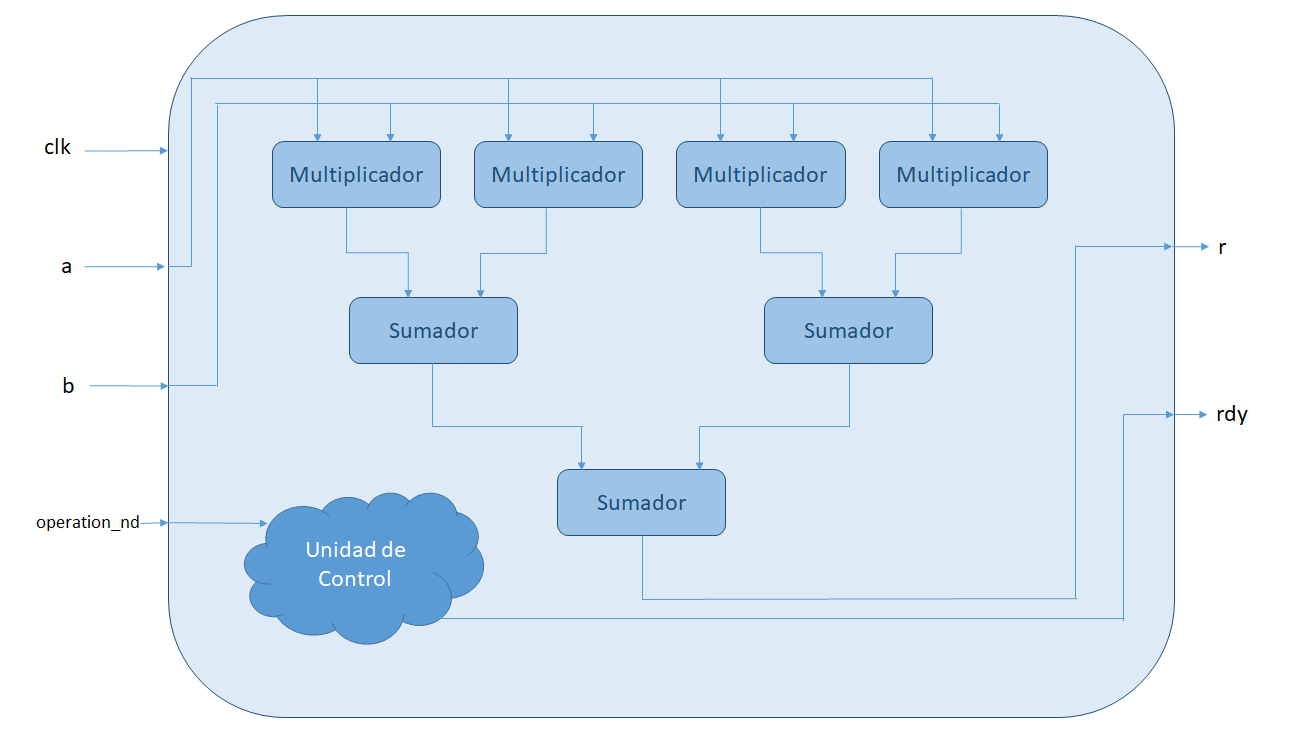
\includegraphics[width=1\textwidth]{Imagenes/DiagramaModuloProductoEscalar.png}
  \caption{Representación gráfica de un ejemplo del módulo Producto Escalar implementado en VHDL.}
  \label{fig:modulo producto escalar vhdl}
\end{figure}

\begin{itemize}
    \item DESCRIPCIÓN
        \begin{itemize}
            \item Realiza el producto escalar de las dos entradas A y B, que serán dos vectores de Nx32 bits. Se utilizan N multiplicadores, uno por cada multiplicación A[i]xB[i], y, posteriormente, un árbol de sumadores conectado a los resultados de los multiplicadores, obteniendo al final un numero de 32 bits que indica el producto escalar de los vectores A y B. Cuando el resultado está disponible, se muestra por la salida r en el siguiente flanco de reloj. Se puede observar gráficamente un ejemplo de este módulo para N = 4 en la Figura~\ref{fig:modulo producto escalar vhdl}.
        \end{itemize}
    \item GENÉRICOS
        \begin{itemize}
            \item N = 4: número de elementos que tiene cada vector. Para el algoritmo no se utilizará este valor, sino el número de bandas.
            \item N$\_$log2 = 2: logaritmo en base 2 de N. Para el algoritmo no se utilizará este valor sino el logaritmo en base 2 del número de bandas.
        \end{itemize}
    \item INPUT
        \begin{itemize}
            \item clk: señal de reloj.
            \item a: señal de Nx32 bits indicando el vector A.
            \item b: señal de Nx32 bits indicando el vector B.
            \item operation$\_$nd: señal que indica si los operandos están disponibles.
        \end{itemize}
    \item OUTPUT
        \begin{itemize}
            \item r: señal de 32 bits indicando el resultado del producto escalar de los vectores A y B.
            \item rdy: señal que indica que el resultado ya se encuentra disponible.
        \end{itemize}
    \item UTILIZADO EN
        \begin{itemize}
            \item ATDCA-GS.
        \end{itemize}
\end{itemize}

\subsubsection{Producto Escalar Auxiliar (mult$\_$sum$\_$aux$\_$PF32Bits.vhd)}

\begin{figure}
  \centering
    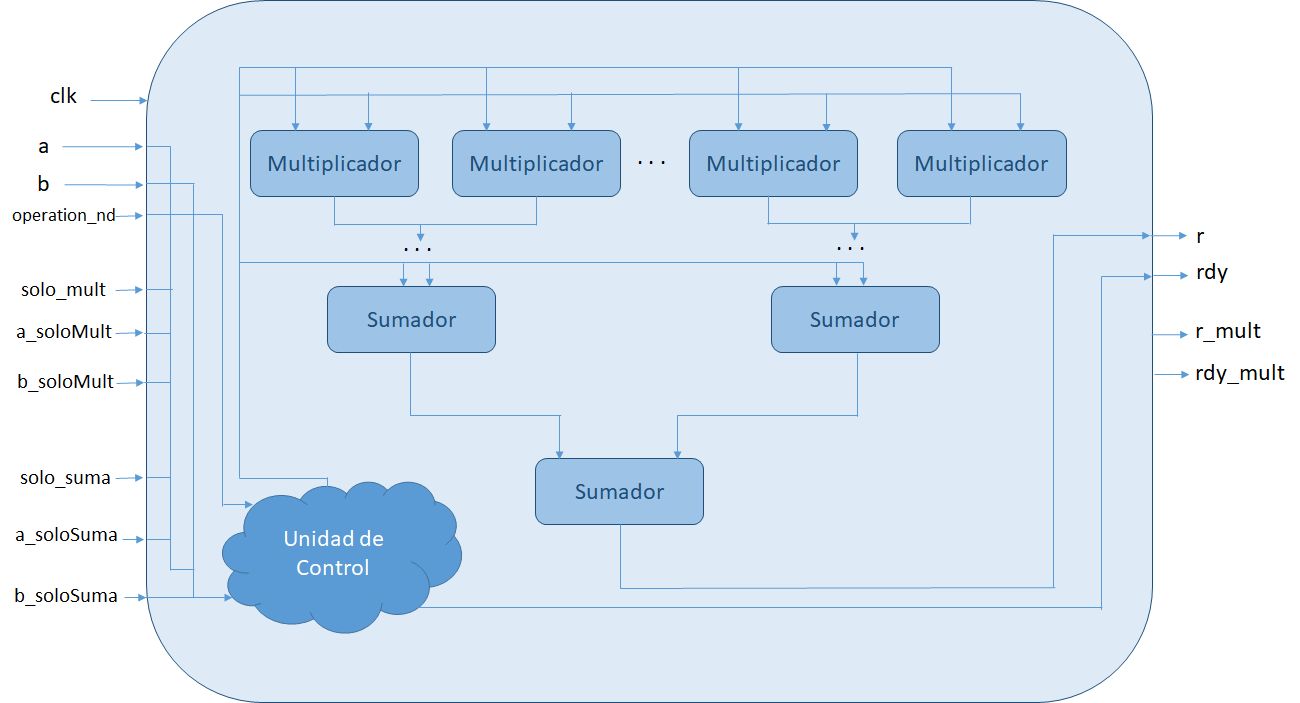
\includegraphics[width=1\textwidth]{Imagenes/DiagramaModuloProductoEscalarAuxiliar.png}
  \caption{Representación gráfica de un ejemplo del módulo Producto Escalar Auxiliar implementado en VHDL.}
  \label{fig:modulo producto escalar auxiliar vhdl}
\end{figure}

\begin{itemize}
    \item DESCRIPCIÓN
        \begin{itemize}
            \item En caso de que solo$\_$suma y solo$\_$mult estén a 0, realiza exactamente la misma funcionalidad que el módulo Producto Escalar. En caso de que solo$\_$suma esté a 1, realiza la suma de todos los elementos de los dos vectores de entrada, A y B, empleando para ello un árbol de sumadores. Cuando el resultado está disponible, se muestra por la salida r en el siguiente flanco de reloj y la señal rdy se pone a 1. En caso de que solo$\_$mult esté a 1, realiza la multiplicación elemento a elemento de los dos vectores de entrada. Cuando se obtiene el resultado, se muestra por la señal r$\_$mult (de Nx32 bits) y la señal rdy$\_$mult se pone a 1. Se puede observar gráficamente un ejemplo de este módulo en la Figura~\ref{fig:modulo producto escalar auxiliar vhdl}.
        \end{itemize}
    \item GENÉRICOS
        \begin{itemize}
            \item N = 256: número de elementos que tiene cada vector (equivaldrá al número de bandas de la imagen).
            \item N$\_$log2 = 8: logaritmo en base 2 de N.
        \end{itemize}
    \item INPUT
        \begin{itemize}
            \item clk: señal de reloj.
            \item a: señal de Nx32 bits indicando el vector A.
            \item b: señal de Nx32 bits indicando el vector B.
            \item operation$\_$nd: señal que indica si los operandos están disponibles.
            \item solo$\_$mult: indica si se debe realizar la multiplicación elemento a elemento o no.
            \item solo$\_$suma: indica si se debe realizar la suma en árbol o no.
            \item a$\_$soloSuma: señal de Nx32 bits indicando el vector A para la operación de suma en árbol.
            \item b$\_$soloSuma: señal de Nx32 bits indicando el vector B para la operación de suma en árbol.
            \item a$\_$soloMult: señal de Nx32 bits indicando el vector A para la operación de multiplicación elemento a elemento.
            \item b$\_$soloMult: señal de Nx32 bits indicando el vector B para la operación de multiplicación elemento a elemento.
        \end{itemize}
    \item OUTPUT
        \begin{itemize}
            \item r: señal de 32 bits indicando el resultado de la operación suma en árbol o la de producto escalar (la que se haya realizado) de los vectores A y B.
            \item rdy: señal que indica que el resultado de la operación suma en árbol o la de producto escalar (la que se haya realizado) ya se encuentra disponible.
            \item r: señal de 32 bits indicando el resultado de la operación de multiplicación elemento a elemento de los vectores A y B.
            \item rdy$\_$mult: señal que indica que el resultado de la operación de multiplicación elemento a elemento ya se encuentra disponible.
        \end{itemize}
    \item UTILIZADO EN
        \begin{itemize}
            \item ATDCA-GS.
        \end{itemize}
\end{itemize}

\subsubsection{Registro (registro$\_$rst.vhd)}

\begin{itemize}
    \item DESCRIPCIÓN
        \begin{itemize}
            \item En cada flanco de reloj, si la señal load está a 1, se introduce el dato de la señal din en el registro. Si está a 0, no se produce esta actualización. Por la señal dout sale lo que haya dentro del registro en cada flanco de reloj con una política de Read First, lo que significa que, si se ha actualizado el contenido del registro (load = 1), será el nuevo dato el que saldrá por dout en ese mismo instante de tiempo. Las señales rst y rst$\_$sync, si están a 1, reinician el registro haciendo que el contenido del mismo sean 0’s.
        \end{itemize}
    \item GENÉRICOS
        \begin{itemize}
            \item n = 32: número de bits de los datos que se almacenan en el registro.
        \end{itemize}
    \item INPUT
        \begin{itemize}
            \item clk: señal de reloj.
            \item rst: señal de reset asíncrona.
            \item rst$\_$sync: señal de reset síncrona.
            \item load: señal que indica si se actualiza el valor del registro o se deja tal y como está.
            \item din: señal de n bits indicando el dato a introducir en el registro.
        \end{itemize}
    \item OUTPUT
        \begin{itemize}
            \item dout: señal de n bits indicando el dato que se encuentra almacenado en el registro.
        \end{itemize}
    \item UTILIZADO EN
        \begin{itemize}
            \item Registro Mayor Valor en el módulo Pixel Más Distinto.
            \item Registro Mayor Posición en el módulo Pixel Mas Distinto.
            \item Registro Auxiliar.
        \end{itemize}
\end{itemize}

\subsubsection{Pixel Más Distinto (pixel$\_$mas$\_$distinto.vhd)}

\begin{figure}
  \centering
    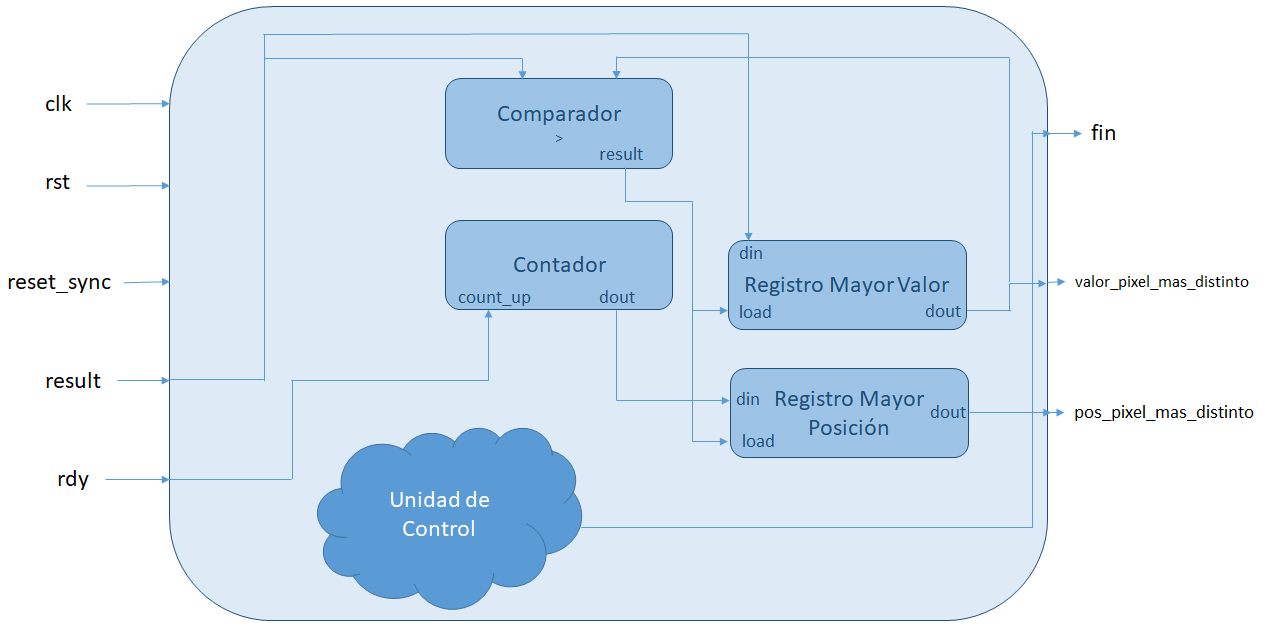
\includegraphics[width=1\textwidth]{Imagenes/DiagramaModuloPixelMasDistinto.png}
  \caption{Representación gráfica del módulo Pixel Más Distinto implementado en VHDL.}
  \label{fig:modulo pixel mas distinto vhdl}
\end{figure}

\begin{itemize}
    \item DESCRIPCIÓN
        \begin{itemize}
            \item Recibe un número de píxeles y calcula cuál de ellos es el más brillante (o distinto), es decir, el que tiene mayor valor. Para ello hace uso de dos registros, un contador y un comparador que indica si el operando A es mayor que el operando B. Se puede observar gráficamente la estructura de este módulo en la Figura~\ref{fig:modulo pixel mas distinto vhdl}.
        \end{itemize}
    \item GENÉRICOS
        \begin{itemize}
            \item NUMPIXELES = 2: número de pixeles que se van a analizar. El algoritmo sobreescribirá este valor según el número de pixeles sobre el que se ejecute.
            \item NUM$\_$PIXELES$\_$log2 = 1: logaritmo en base dos del número de píxeles. El algoritmo sobreescribirá este valor según el número de pixeles sobre el que se ejecute.
        \end{itemize}
    \item INPUT
        \begin{itemize}
            \item clk: señal de reloj.
            \item rst: señal de reset asíncrona.
            \item reset$\_$sync: señal de reset síncrona.
            \item result: señal de 32 bits indicando el siguiente pixel a analizar.
            \item rdy: señal que indica que el siguiente pixel a analizar ya se encuentra disponible.
        \end{itemize}
    \item OUTPUT
        \begin{itemize}
            \item fin: señal que indica que ya se han analizado todos los píxeles y ya se ha encontrado el pixel más distinto.
            \item pos$\_$pixel$\_$mas$\_$distinto: señal de NUM$\_$PIXELES$\_$log2 bits que indica la posición en la memoria del pixel más distinto que se ha encontrado.
            \item valor$\_$pixel$\_$mas$\_$distinto: señal de 32 bits que indica el valor del pixel más distinto que se ha encontrado.
        \end{itemize}
    \item UTILIZADO EN
        \begin{itemize}
            \item ATDCA-GS.
        \end{itemize}
\end{itemize}

\subsubsection{Array Resta con Acumulación (array$\_$restadores$\_$con$\_$acumulacion$\_$PF32Bits.vhd)}

\begin{figure}
  \centering
    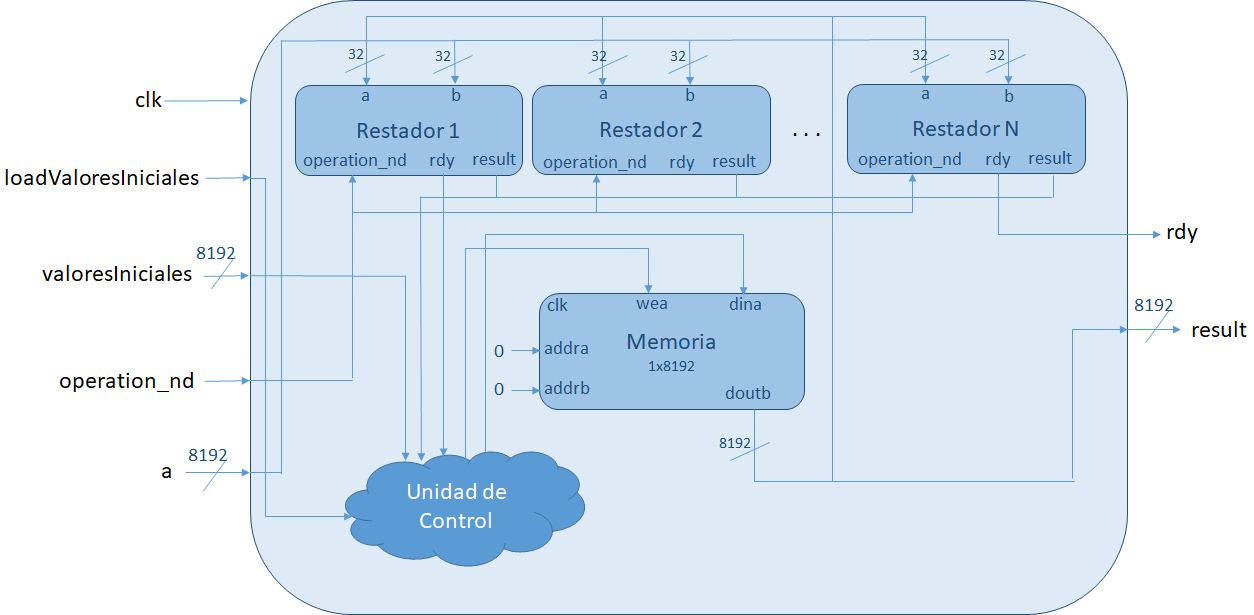
\includegraphics[width=1\textwidth]{Imagenes/DiagramaModuloArrayRestaConAcumulacion.png}
  \caption{Representación gráfica del módulo Array Resta Con Acumulación implementado en VHDL.}
  \label{fig:modulo array resta con acumulacion vhdl}
\end{figure}

\begin{itemize}
    \item DESCRIPCIÓN
        \begin{itemize}
            \item Recibe un operando de Nx32 bits y lo resta a un valor que puede ser, o bien un valor inicial cargado previamente a los cálculos, o bien el resultado acumulado de las operaciones anteriores. La resta se realiza como si fuera una operación elemento a elemento de dos vectores de N números en punto flotante, por lo que se utilizan N restadores. Para almacenar el valor acumulado se hace uso de una memoria de 1x8192 bits. Se puede observar gráficamente la estructura de este módulo en la Figura~\ref{fig:modulo array resta con acumulacion vhdl}.
        \end{itemize}
    \item GENÉRICOS
        \begin{itemize}
            \item N = 256: número de restadores que se van a utilizar (el equivalente al número de bandas de la imagen hiperespectral).
        \end{itemize}
    \item INPUT
        \begin{itemize}
            \item clk: señal de reloj.
            \item loadValoresInciales: señal que indica si se cargan los valores iniciales o no.
            \item valoresInciales: señal de Nx32 bits que representa los valores iniciales que deben cargarse cuando sea necesario.
            \item operation$\_$nd: señal que indica si los operandos están disponibles para las restas.
            \item a: señal de Nx32 bits que representa los N elementos que se desean restar a los valores acumulados hasta el momento.
        \end{itemize}
    \item OUTPUT
        \begin{itemize}
            \item result: señal de Nx32 bits indicando el resultado de las operaciones.
            \item rdy: señal que indica que el resultado de las operaciones ya se encuentra disponible.
        \end{itemize}
    \item UTILIZADO EN
        \begin{itemize}
            \item ATDCA-GS.
        \end{itemize}
\end{itemize}

\section{Paralelización y optimización del algoritmo ATDCA-GS usando OpenCL}

Se ha realizado el estudio de una implementación paralela del algoritmo usando el paradigma OpenCL para su posterior optimización\footnote{https://www.intel.com/content/dam/www/programmable/us/en/pdfs/literature/hb/opencl-sdk/aocl-best-practices-guide.pdf}. Antes de continuar con el estudio, se comentará una serie de conceptos relacionados con el paradigma de progrmación OpenCL.

La especificación de OpenCL\footnote{https://www.khronos.org/opencl} fue desarrollada para permitir una libertad en términos de implementar aplicaciones que podrían ejecutarse en diferentes arquitecturas. En el paradigma OpenCL, el programa ``host'', está a cargo de las operaciones de E/S, inicialización de datos y controlando el ``device''. Además, lanza los códigos ``kernel'' y la sincronización entre ellos. Entre los principales beneficios se encuentra el amplio rango de dispositivos hardware a ser usados: CPUs, GPUs y FPGAs. Todos ellos podrán ser usados con un esfuerzo moderado en el proceso de codificación.

\begin{figure}[htb]
\centering
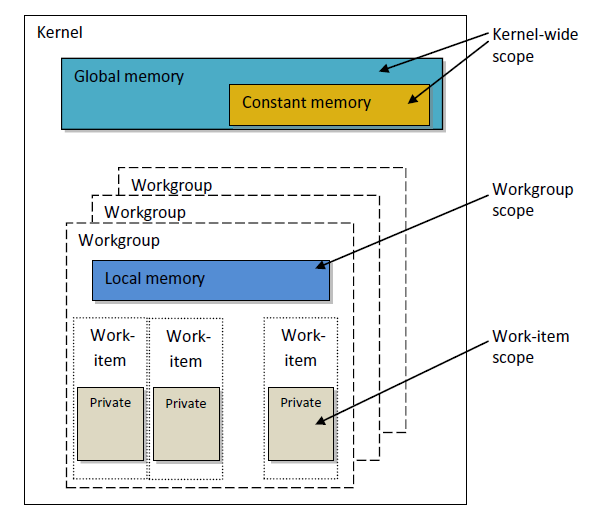
\includegraphics[width=0.75\textwidth]{images/imagen_jerarquia.PNG}
\caption{Jerarquía de memoria en OpenCL, y división en \textit{work-items}.} \label{fig:imagen_jerarquia}
\end{figure}

Un kernel OpenCL permite expresar paralelismo a través de la ejecución de varios \textit{work-items}. Un grupo de \textit{work-items} forman un textit{work-group} que corre sobre una unidad de cómputo individual o ``single compute unit''. Los \textit{work-items} ejecutan el mismo \textit{kernel}  (con un único id), comparte una memoria rápida denominada \textit{local memory} (ver Figura \ref{fig:imagen_jerarquia}\footnote{https://www.mql5.com/es/articles/407}) y puede ser sincronizada con barreras. La dimensión máxima de cada {work-group} dependerá de la especificación del \textit{device} usado (ver Sección \ref{ch:chapte5}).   

Una vez que se han conocido los conceptos relacionados con el paradigma de programación paralela OpenCL, pasaremos a analizar una implementación previa en OpenCL del algoritmo ATDCA-GS. En este trabajo previo \cite{portabilitySPIE_Sergio} fueron implementados tres kernels: cálculo del píxel más brillante, cálculo de la proyección ortogonal de cada píxel sobre la imagen y obtención de la máxima proyección ortogonal. De cada uno de ellos se mostrará a continuación el pseudocódigo que se ha seguido.

%Para su implementación en OpenCL se ha realizado un perfilado del código optimizado en lenguaje C. A través de este estudio se ha podido encontrar las distintas porciones de código candidatas a paralelizar, ya que podrían llegar a ser posibles cuellos de botella de rendimiento o también conocido como "bottlenecks". Se han encontrado hasta un total de 3 zonas de códigos donde una correcta paralelización puede suponer una mejora en el rendimiento. Estas zonas son: cálculo del píxel más brillante, cálculo de la proyección ortogonal de un píxel sobre la imagen y obtención de la máxima proyección ortogonal. Para cada una de las zonas identificadas, un \textit{kernel} será implementado.

El primer \textit{kernel} sobre el que se ha realizado el estudio, es el correspondiente al cálculo del píxel más brillante. El pseudocódigo estudiado es el descrito en el algoritmo \ref{kernel_brightest_opencl}. Tras analizarlo y teniendo en cuenta que esta parte consume aproximadamente el \textbf{5\%} del tiempo de procesamiento total del algoritmo considerando una imagen hiperespectral real como es Cuprite, se han tenido en cuenta varias consideraciones: 

\begin{algorithm}[htb]\small
\caption{Cálculo del píxel más brillante}
\begin{algorithmic}[1]
\label{kernel_brightest_opencl}
\STATE global d$\_$image $\leftarrow{}$ Vector inicial $\textbf{X}$$[r]$, d$\_$bright $\leftarrow{}$ El valor brillo de cada píxel\\
\STATE registers bright $\leftarrow{}$ 0, value $\leftarrow{}$ 0\\
\STATE id $\leftarrow{}$ get\_group\_id(0) * get\_local\_size(0) +
get\_local\_id(0)\\
\% $n_{b}$ indica el número de bandas espectrales\\ 
\IF{$id < r$} 
\FOR{$k=0 \text{ to } n_{b}$}
\STATE value $\leftarrow{}$ d$\_$image[id + (k * r)]\\
\STATE bright $\leftarrow{}$ bright + value * value\\
\ENDFOR 
\STATE d$\_$bright[id] $\leftarrow{}$ bright\\
\ENDIF
\end{algorithmic}
\end{algorithm}

\begin{enumerate}
\item Empleo de \textit{restrict} en arrays usados en memoria global. De esta manera se evita que los punteros no estén apuntando a ubicaciones en memoria con información. A la hora de definir los parámetros de la función kernel se ha acompañado la variable \textit{restrict} a los arrays declarado en memoria global (\textit{restrict d\_image} y \textit{restrict d\_bright}).
%\item Uso de relleno adicional o \textit{padding} en arrays.
\item Distribución óptima de los datos para favorecer la vectorización. Para ello, la línea 6 del Algoritmo \ref{kernel_brightest_opencl} se ha modificado por lo siguiente: d$\_$image[k + (id * $n_{b}$)].
\item Desenrollado de bucles (\textit{loop unrolling}). Entre las líneas 4 y 5 del Algoritmo \ref{kernel_brightest_opencl} se ha introducido la siguiente directiva: \#\textit{pragma unroll num\_factor}, permitiendo un factor diferente para el desenrollado del bucle dependiendo del tamaño de la imagen. 
\end{enumerate}

\begin{algorithm}[htb]\small
\caption{Reducción para obtener la máxima proyección ortogonal}
\begin{algorithmic}[1]
\label{kernel_reduction}
\STATE global d$\_$bright, d$\_$projection, d$\_$index\\
\STATE local s$\_$p[BLK] $\leftarrow{}$Estructura inicial para almacenar todas las proyecciones\\
\STATE local s$\_$i[BLK] $\leftarrow{}$Estructura inicial para almacenar todos los índices para cada proyección\\
\STATE tid $\leftarrow{}$ get\_local\_id(0)\\
\STATE id $\leftarrow{}$ get\_group\_id(0)  * (get\_local\_size(0) * 2) + get\_local\_id(0)\\
\IF{(id + get\_local\_size(0)) $\ge$ r}
	\STATE s$\_$p[tid] $\leftarrow{}$ d$\_$bright[id]
	\STATE s$\_$i[tid] $\leftarrow{}$ id
\ELSE
	\IF{d$\_$bright[id] $>$ d$\_$bright[id + get\_local\_size(0)]}
		\STATE s$\_$p[tid] $\leftarrow{}$ d$\_$bright[id]
		\STATE s$\_$i[tid] $\leftarrow{}$ id
    \ELSE
    	\STATE s$\_$p[tid] $\leftarrow{}$ d$\_$bright[id + get\_local\_size(0)]
		\STATE s$\_$i[tid] $\leftarrow{}$ (id + get\_local\_size(0))
	\ENDIF
\ENDIF

\STATE barrier($\text{CLK\_LOCAL\_MEM\_FENCE}$)\\

\% En esta sincronización, todos los hilos deben esperar la ejecución de todos los hilos en un bloque para poder completar la copia en memoria local de s$\_$p y s$\_$i

\FOR{s=get\_local\_size(0) / 2 $\text{ to }$ {s$>$0; s$>>$=1}}
	\IF{tid $<$ s}
    	\IF{s$\_$p[tid] $\le$ s$\_$p[tid + s]}
    		\STATE s$\_$p[tid] $\leftarrow{}$ s$\_$p[tid + s]
			\STATE s$\_$i[tid] $\leftarrow{}$ s$\_$i[tid + s]
		\ENDIF
    \ENDIF
    \STATE barrier($\text{CLK\_LOCAL\_MEM\_FENCE}$)\\
\ENDFOR
\STATE d$\_$projection[get\_group\_id(0)] $\leftarrow{}$ s$\_$p[0]\\
\STATE d$\_$index[get\_group\_id(0)] $\leftarrow{}$ s$\_$i[0]\\
\STATE barrier($\text{CLK\_LOCAL\_MEM\_FENCE}$)\\
\end{algorithmic}
\end{algorithm}

El siguiente \textit{kernel} que ha sido analizado es la reducción para obtener la máxima proyección ortogonal. El pseudocódigo estudiado es el descrito en el Algoritmo \ref{kernel_reduction}. Tras analizarlo, se ha llegado a la conclusión de que no se podrían realizar grandes optimizaciones en este kernel ya que el tiempo de ejecución exclusivamente de esta parte está por debajo del \textbf{2\%} del tiempo total del algoritmo usando una imagen real como es Cuprite.

Por último, nos encontramos con el kernel que se encarga de computar la proyección ortogonal de cada uno de los píxeles que conforman la imagen. El pseudocódigo estudiado es el descrito en el Algoritmo \ref{pixel_projection}. Esta parte del código constituye aproximadamente un \textbf{90\%} en cuanto al tiempo de procesamiento total del algoritmo. La parte más costosa la podemos encontrar entre las líneas 18-21. Al igual que en el primer kernel, se ha optado por las mismas consideraciones: empleo de la variable \textit{restrict}, distribución óptima de los datos para favorecer la vectorización y por supuesto, un desenrollado de este bucle que depende del número de bandas espectrales usado. Para ello, se han realizado las siguientes modificaciones al Algoritmo  \ref{pixel_projection}:

\begin{algorithm}[htb]\small
\caption{Cálculo de las proyecciones ortogonales para cada píxel}
\begin{algorithmic}[1]
\label{pixel_projection}
\STATE global d$\_$image $\leftarrow{}$ Vector inicial $\textbf{X}[r]$\\ 
\STATE global d$\_$projection $\leftarrow{}$ El valor proyección para cada píxel ${x}_{i}$ en $\textbf{X}$\\
\STATE global d$\_$f $\leftarrow{}$ The vector más ortogonal\\
\STATE registers sum $\leftarrow{}$ 0, value $\leftarrow{}$ 0\\
\STATE local s$\_$df[$n_{b}$] $\leftarrow{}$ Estructura inicial $\textbf{d\_f}$ con el vector más ortogonal\\
%\STATE id $\leftarrow{}$ get\_group\_id(0) * get\_local\_size(0) + get\_local\_id(0)\\
\STATE id $\leftarrow{}$ get\_global\_id(0)\\
\IF{$id < r$}
	\IF{$get\_local\_size(0) < {n_{b}}$} 
		\FOR{$i=get\_local\_id(0) \text{ to } {n_{b}}$}
			\STATE s$\_$df[i] $\leftarrow{}$ d$\_$f[i]
		\ENDFOR 
	\ELSE
		\IF{$get\_local\_id(0) < {n_{b}}$}
			\STATE s$\_$df[get\_local\_id(0)] $\leftarrow{}$ d$\_$f[get\_local\_id(0)]\\
		\ENDIF
	\ENDIF
	\STATE barrier($\text{CLK\_LOCAL\_MEM\_FENCE}$)
	%\% In this barrier, all work-items must wait the execution of all work-items in
	%a work-group to complete the copy in local memory of $d\_f$
	\% Espera hasta que la copia de $d\_f$ se haya completado en memoria local
	\FOR{$i=0 \text{ to } {n_{b}}$}
		\STATE value $\leftarrow{}$ d$\_$image[id + (i * r)]\\
		\STATE sum $\leftarrow{}$ sum + value * s$\_$df[i]\\
	\ENDFOR
	\STATE d$\_$projection[id] $\leftarrow{}$ sum * sum\\
\ENDIF
\end{algorithmic}
\end{algorithm}

\begin{enumerate}
    \item Se ha declarado la variable \textit{restrict} a los arrays usados en memoria global (\textit{restrict d\_image}, {restrict d\_projection} y {restrict d\_f}).
    %\item Uso de padding en arrays.
    \item Se ha empleado otra distribución de los datos para favorecer la vectorización. La línea 19 del Algoritmo \ref{pixel_projection} ha sido modificada con lo siguiente: d$\_$image[i + (id * $n_{b}$)].
    \item Uso óptimo del desenrollado de bucles. Entre las líneas 17 y 18 del Algoritmo \ref{pixel_projection} se ha introducido la siguiente directiva: \#\textit{pragma unroll num\_factor}, permitiendo un factor diferente para el desenrollado del bucle dependiendo del tamaño de la imagen.  
\end{enumerate}

Las optimizaciones aplicadas a los kernels descritos anteriormente han favorecido que el tiempo de procesamiento sea menor aumentando el rendimiento de nuestra implementación. El análisis será cubierto en el capítulo siguiente.
    %\cleardoublepage
%\thispagestyle{empty}
\mbox{}

\chapter{Resultados}
\label{ch:chapte5}

\section{Conjunto de datos hiperespectrales}

Para realizar los experimentos, se han utilizado diferentes conjuntos de datos hiperespectrales, tanto reales como sintéticos:

\begin{figure}
\centering
\begin{tabular}{cc}
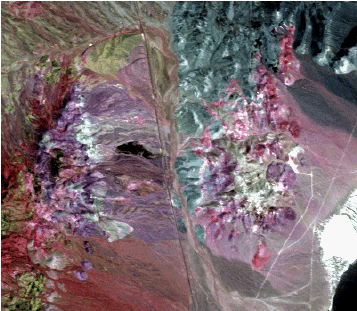
\includegraphics[height=0.35\textwidth]{images/cupritecolor.png} &
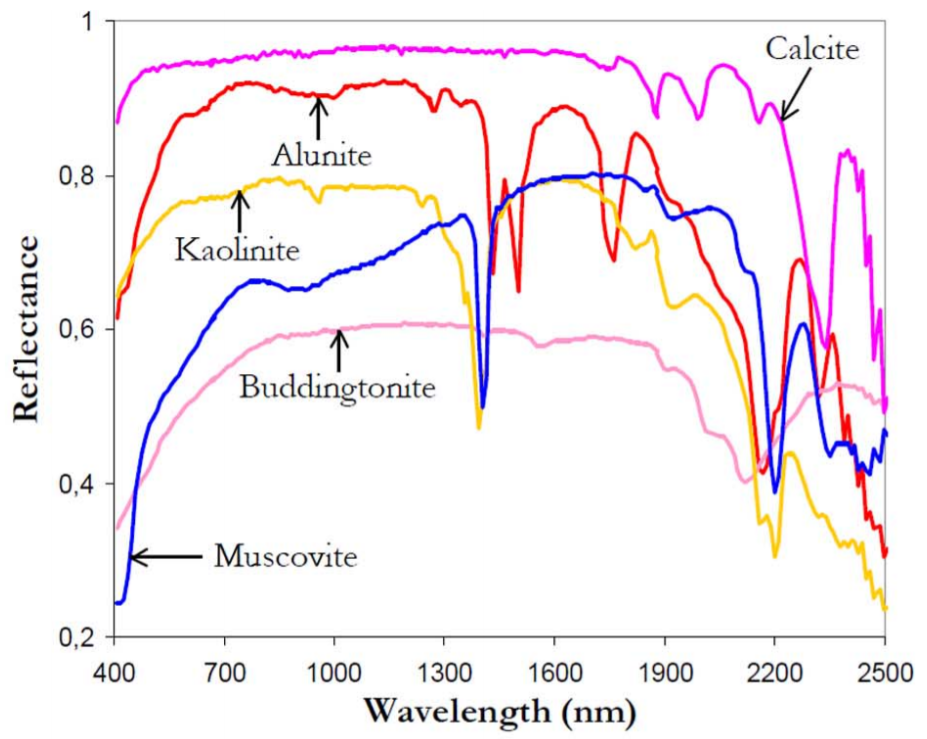
\includegraphics[height=0.35\textwidth]{images/cupriteSignatures.png}\\
(a) & (b)\\
\end{tabular}
\caption{(a) Composición en falso color de la escena captada por el sensor hiperespectral AVIRIS sobre el distrito minero de Cuprite en Nevada. (b) Firmas espectrales de la biblioteca U.S. Geological Survey de los minerales expuestos de interés.} \label{fig:aviriscuprite}
\end{figure}

\begin{itemize}
    \item El primer conjunto de datos corresponde a la conocida escena AVIRIS Cuprite (ver Figura \ref{fig:aviriscuprite}(a)), recogida en el verano de 1997 y disponible online en unidades de reflectancia después de ser corregida atmosféricamente. La porción utilizada en los experimentos corresponde a un subconjunto de 350 x 350 píxeles del sector, etiquetados como f970619t01p02\_r02\_sc03.a.rfl en los datos online, que cuenta con 224 bandas espectrales en el rango de 400 a 2500 nanómetros y un tamaño total de alrededor de 50 megabytes. Las bandas 1-3, 105-115 y 150-170 han sido eliminadas antes del análisis debido a la absorción por agua y la baja relación señal-ruido o signal-to-noise ratio (SNR) de estas bandas. La zona es bien conocida mineralógicamente, y tiene varios minerales expuestos de interés, incluyendo alunita, buddingtonita, calcita, caolinita y moscovita. Las firmas de referencia de suelo de los minerales mencionados (ver Figura \ref{fig:aviriscuprite}(b)), disponibles en la biblioteca U.S. Geological Survey library (USGS), se utilizarán para evaluar la pureza de la firma de los endmembers en este trabajo.
    
    \item El segundo conjunto de datos corresponde a una imagen sintética (ver Figura \ref{figure:synthetic}) que nos ayudará a evaluar la escalabilidad de nuestras implementaciones. La imagen ha sido construida usando un conjunto de 30 firmas espectrales de la librería USGS y el procedimiento descrito en \cite{miller1986definition} para simular patrones naturales espaciales. La imagen sintética resultante está compuesta por un total de 750$\times$650 píxeles y 224 bandas espectrales, dando como resultado un tamaño aproximado de 437 MB. La Figura \ref{figure:synthetic} muestra una composición en falso color de la escena simulada y tres ejemplos de mapas de abundancia verdad terreno (construidos a partir de píxeles puros o endmembers).
    
\end{itemize}

\begin{figure}[ht]
\centering
\begin{tabular}{cc}
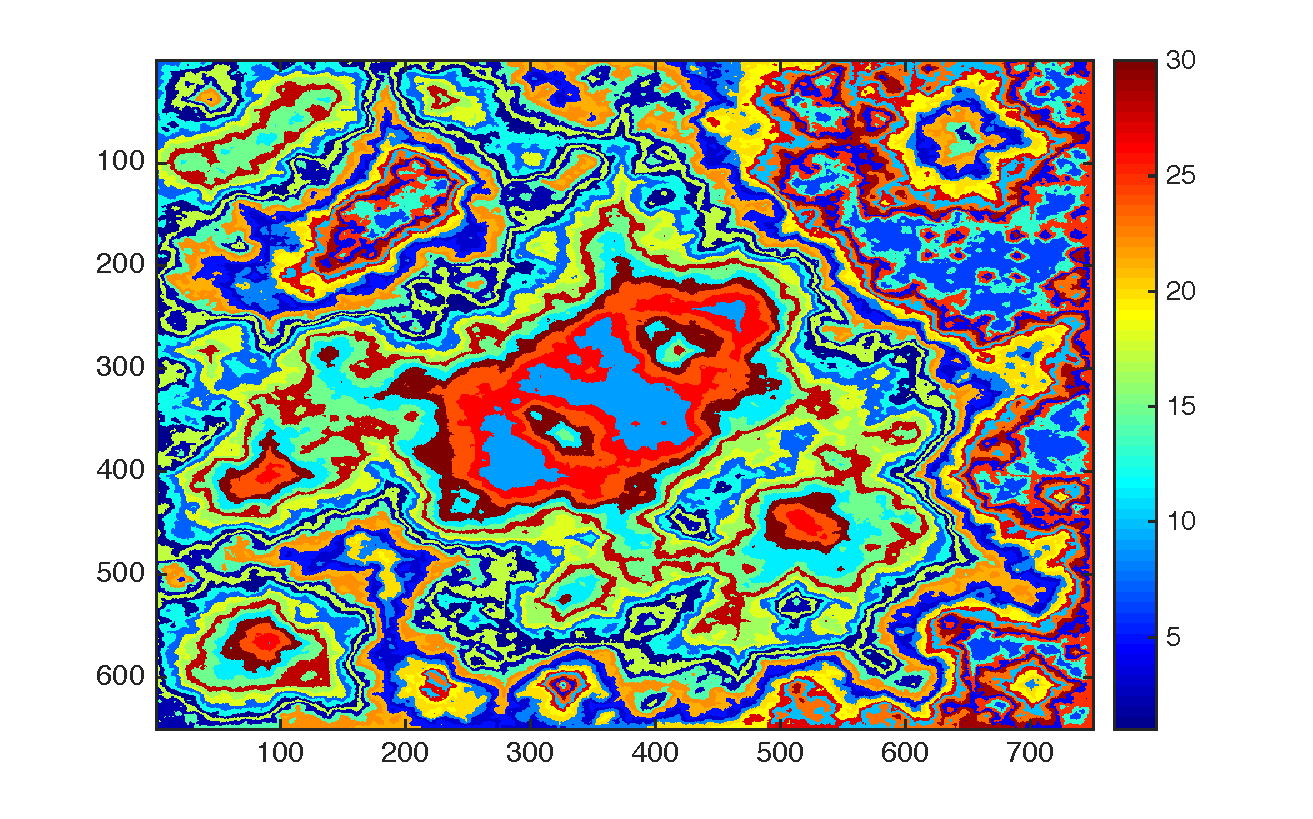
\includegraphics[height=0.30\textwidth]{./images/Synthetic1.pdf} &
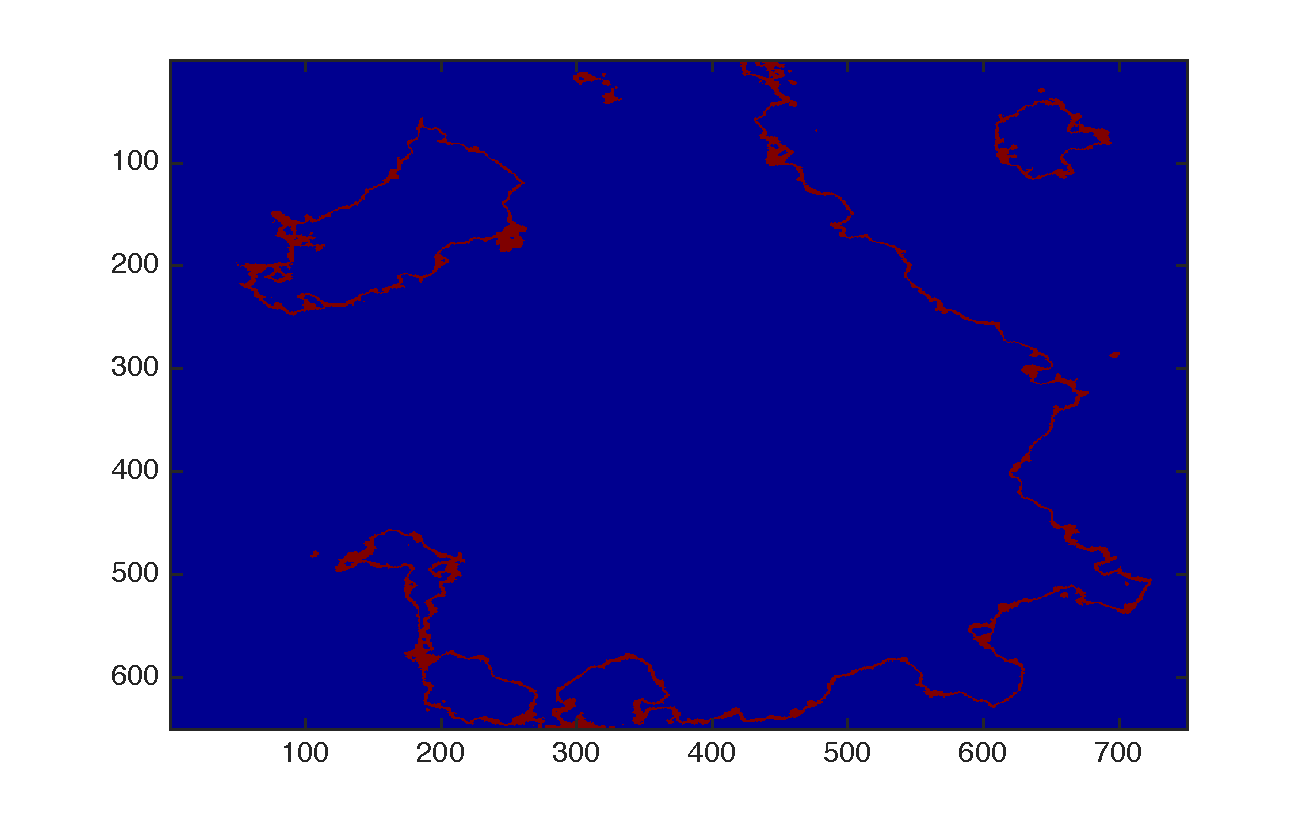
\includegraphics[height=0.30\textwidth]{./images/Synthetic1_end_3.pdf}\\
(a) & (b)\\
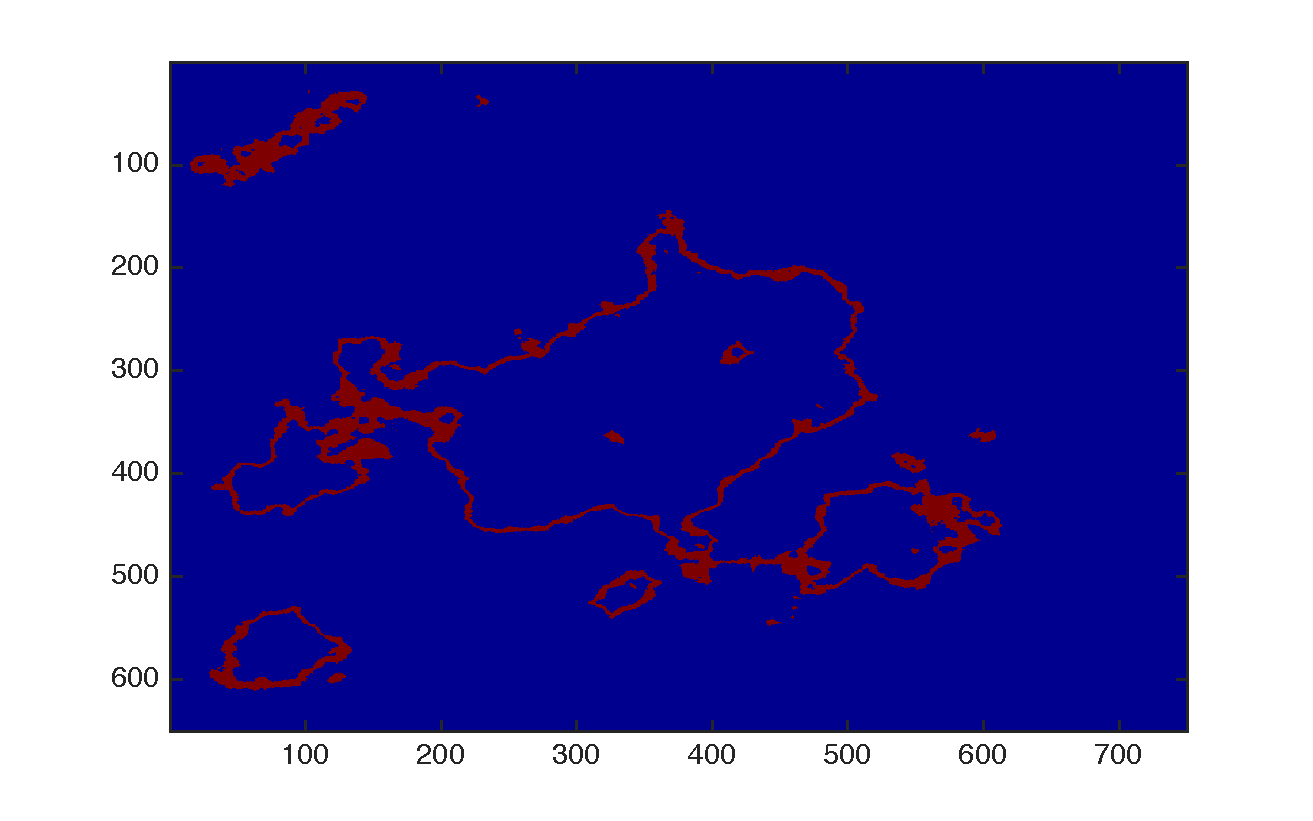
\includegraphics[height=0.30\textwidth]{./images/Synthetic1_end_15.pdf} &
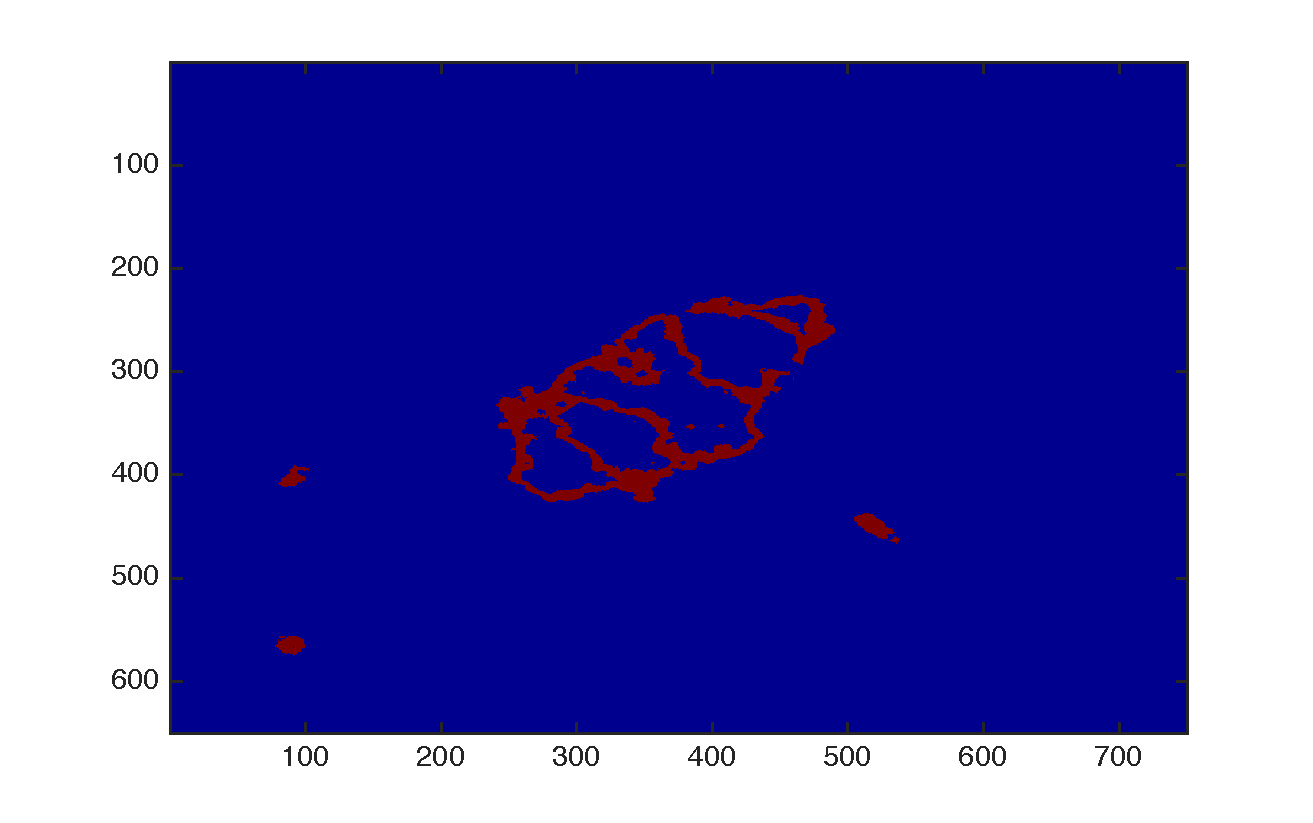
\includegraphics[height=0.30\textwidth]{./images/Synthetic1_end_26.pdf}\\
(c) & (d)\\
\end{tabular}
\caption{(a) Composición en falso color de la escena sintética. (b) Endmember \#3. (c) Endmember \#15. (d) Endmember \#26.}
\label{figure:synthetic}
\end{figure}

\section{Plataformas FPGAs}

\begin{figure}
  \centering
    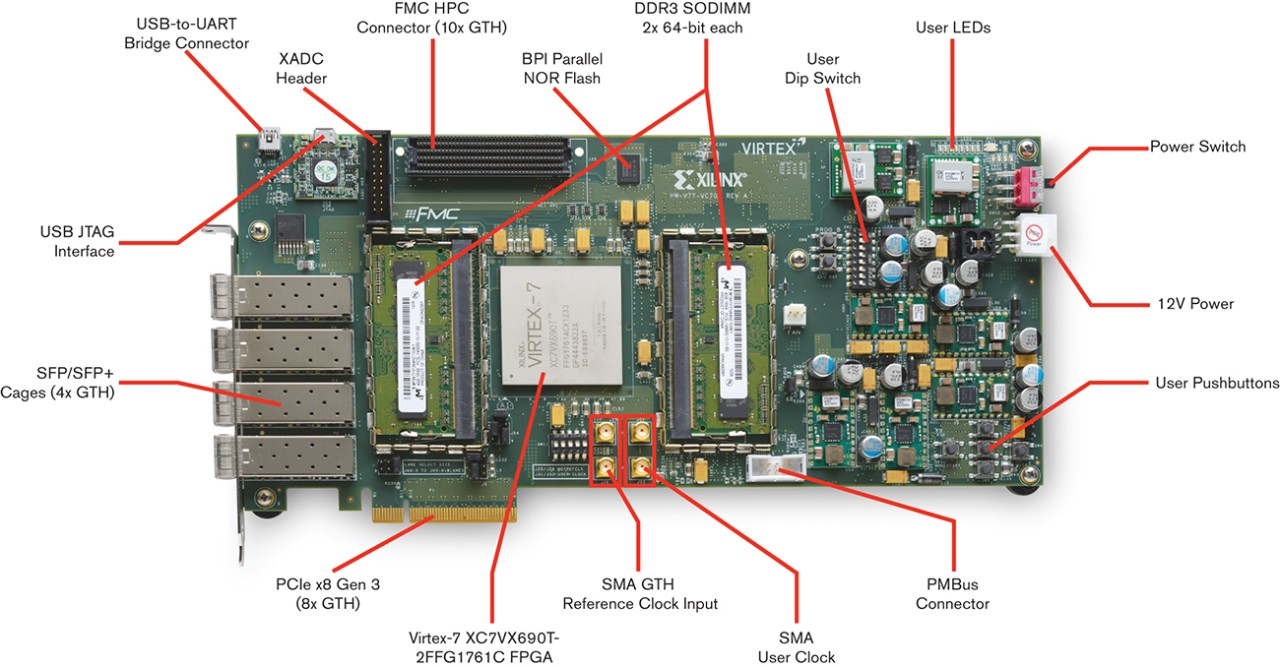
\includegraphics[width=1\textwidth]{images/VC709.png}
  \caption{Placa VC709.}
  \label{fig:VC709}
\end{figure}

\begin{figure}
  \centering
    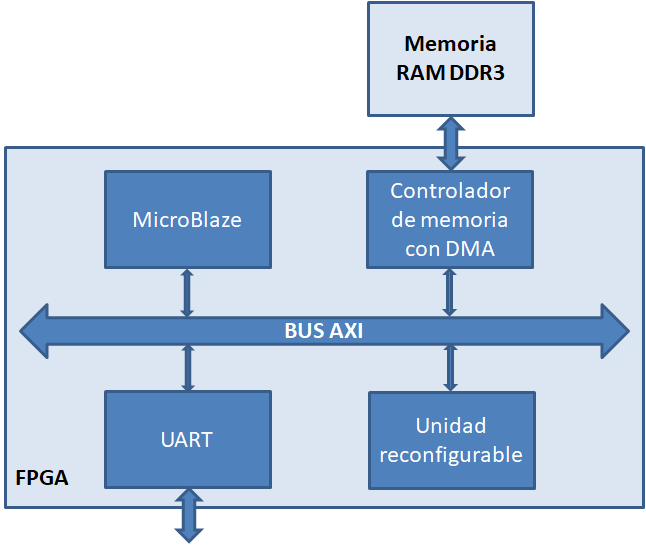
\includegraphics[width=0.7\textwidth]{images/plataforma_test.png}
  \caption{Plataforma de test para la placa VC709.}
  \label{fig:plataforma de test}
\end{figure}

El algoritmo completo en VHDL se ha implementado en una placa VC709 (ver Figura \ref{fig:VC709}), una placa reconfigurable con una sola Virtex-7 XC7VX690T, dos ranuras DDRM DDR3 que admiten hasta 4 GB cada una, un puerto RS232 y algunos componentes adicionales que no se han utilizado en nuestra implementación. La FPGA de Xilinx Virtex-7 XC7VX690T tiene una capacidad total de 693,120 celdas lógicas, 3,600 DSPs y 52,920 Kb de memoria.


Para llevar a cabo la validación del algoritmo en placa, se ha utilizado la plataforma de test que se muestra en la Figura \ref{fig:plataforma de test}. Como se puede observar, consta de un microprocesdor tipo MicroBlaze, un controlador de memoria, un puero serie y una unidad reconfigurable, todo ello interconectado mediante el bus AXI. Dentro de la unidad reconfigurable, se ubicaría el algoritmo a testear.

Por otro lado, para la implementación en OpenCL se ha hecho uso de la FPGA Intel Arria 10 GX 10AX115S2F45I2SGES (ver Tabla \ref{Arria10} para conocer los recursos disponibles y las particulariedades sobre el modelo de memoria en OpenCL). Este dispositivo se encuentra instalado en un servidor con un procesador Intel Xeon E5-1620 v3, con 4 cores físicos cada uno a una frecuencia de reloj de 3.5GHz y 64GB de memoria RAM DDR3. El sistema operativo empleado en este servidor es un CentOS Linux 7 y cuenta con la versión 17.1.0 del Intel FPGA SDK for OpenCL Offline Compiler.

\begin{table}[htb]
	\centering
	\begin{tabular}{|l|c|c|c|}
		\hline
		 & OpenCL & FPGA & Intel Arria 10 GX\\
		 \hline \hline
		 Memoria & Global & External &2GB DDR3\\ \hline 
		 & Constant &  Cache & 32KB DDR3\\ \hline 
		 & Local & Embedded & 67Mbits\\ \hline 
		 & Private & Registers & 67244Kbits \\ \hline
	\end{tabular}
	\caption{Modelo de memoria en OpenCL y recursos disponibles para la FPGA Intel Arria 10 GX.}
	\label{Arria10}
\end{table}

\section{Métricas}

\subsection{Calidad}
Antes de describir los resultados obtenidos, se describe primero la métrica utilizada para la comparación cuantitativa en los experimentos realizados. Con el fin de reducir el impacto de las fuentes de interferencia atmosférica en la evaluación realizada, se utiliza el ángulo espectral (AE) entre el endmember más similar detectado por la implementación propuesta y la firma espectral de referencia disponible en cada escena. El AE entre un píxel $X(i, j)$ seleccionado por el algoritmo ATGP-GS y una firma espectral de referencia $Si$ disponible a priori, puede calcularse simplemente como:

\begin{equation}\label{eq:ae}
AE[X(i,j), S_i] = cos^{-1} \frac{X(i,j) \cdot S_i}{|X(i,j)| \cdot |S_i|}
\end{equation}

es decir, el AE mide el ángulo formado por dos vectores n-dimensionales. Como resultado, valores bajos de AE significan una alta similitud espectral entre los vectores comparados. Esta medida de similitud espectral es independiente de la multiplicación de $X(i, j)$ y $Si$ por constantes y, en consecuencia, es independiente ante escalas multiplicativas desconocidas que puedan surgir debido a las diferencias en la iluminación y al ángulo de incidencia. Esto nos puede ayudar a compensar las diferentes condiciones de adquisición para un píxel en la imagen original y para una firma espectral recogida sobre el terreno (como es el caso de las firmas de referencia de la librería USGS utilizadas para la imagen AVIRIS Cuprite).

\subsection{Rendimiento}

Para medir el rendimiento se ha tenido en cuenta la aceleración del algoritmo en un lenguaje respecto al otro (ecuación~\ref{eq:metrica rendimiento}) y de esta manera realizar una comparativa entre ambos. Además, se ha identificado cuál es el tiempo límite (máximo) para que el procesamiento del desmezclado espectral de la imagen completa se pueda realizar en tiempo real \cite{tfg_miguel_carlos}, que es uno de los principales objetivos que se persigue en este trabajo.

\begin{equation}\label{eq:metrica rendimiento}
\text{Rendimiento} = \frac{\text{Tiempo OpenCL}}{\text{Tiempo VHDL}}
\end{equation}

%[SergioIni] Habría que darle una vuelta a este párrafo [SergioFin]

Pese a que las pruebas se realizarán sobre imágenes de un tamaño relativamente pequeño, es preciso destacar que si éstas se pueden procesar en tiempo real, las de mayor tamaño también se podrán procesar de esta forma. Esto se debe a que el aumento en el tiempo respecto al tamaño de la imagen es logarítmico, es decir, aumenta poco ante variaciones en el tamaño de las imágenes y/o en el número de endmembers a calcular.

Para medir el rendimiento, primero se analizará el rendimiento en cuanto a recursos empleados en cada implementación con la siguiente metodología: primero, se prestará atención a los recursos empleados (LUTs, LUTRAMs, BRAMs y DSPs) en la FPGA Virtex 7 XC7VX690T con el algorirmo en VHDL para imágenes de 188, 224 y 256 bandas, y se comparará con respecto a los máximos disponibles que ofrece el dispositivo; después, se realizará el mismo análisis pero respecto a la FPGA Intel Arria 10 GX y sus recursos (ALUTs, FFs, RAMs y DSPs), usando primero el algoritmo en OpenCL sin optimizaciones a modo de referencia y después con ellas.

Una vez determinado el rendimiento en cuanto a recursos utilizados, se procederá a evaluar el rendimiento en cuanto a tiempo. En primer lugar, se inferirá una fórmula que calcule el número de ciclos necesarios para analizar cualquier imagen a través del algoritmo en VHDL. Después se analizarán los tiempos de ejecución de las dos implementaciones con la imagen de Cuprite prestando atención para ello a la frecuencia de reloj. A continuación se establecerá una comparativa entre el tiempo teórico máximo alcanzable para un análisis a bordo y el tiempo real que tarda en ejecutarse el algoritmo en los lenguajes VHDL y OpenCL con la penalización de E/S. Finalmente con esta información se afirmará si se consigue viabilidad para un análisis en tiempo real o no.

\section{Resultados experimentales}

\subsection{Calidad}

\begin{table}[htbp]
	\centering
	\begin{tabular}{|l|c|c|}
		\hline
		Mineral en USGS & Implementación & Implementación \\
		 & OpenCL en FPGA & VHDL en FPGA \\ \hline \hline
		Alunita & 5.48$^{\circ}$ & 5.48$^{\circ}$ \\ \hline 
		Buddingtonita & 4.08$^{\circ}$ & 4.08$^{\circ}$ \\ \hline 
		Calcita & 5.87$^{\circ}$ & 5.87$^{\circ}$ \\ \hline 
		Kaolinita & 11.14$^{\circ}$ & 11.14$^{\circ}$ \\ \hline 
		Moscovita & 5.68$^{\circ}$ & 5.68$^{\circ}$ \\ \hline 
	\end{tabular}
	\caption{Ángulo espectral entre los endmembers extraídos en la escena AVIRIS Cuprite por las diferentes implementaciones de ATGP-GS y las firmas de referencia seleccionadas de la librería USGS.}
	\label{tabla2}
\end{table}

En la Tabla~\ref{tabla2} se muestra la calidad de los resultados experimentales tras la ejecución del algoritmo en OpenCL y en VHDL. Cabe señalar que sólo refleja la menor puntuación de AE de todos los endmembers extraídos con respecto a su firma de referencia en cada caso. Dado que se obtienen los mismos resultados, validamos que las dos implementaciones son correctas.

\subsection{Rendimiento}

En la Tabla~\ref{utilization virtex7} se pueden observar los resultados de ocupación en la FPGA Virtex-7 XC7VX690T, a partir de los cuales se puede afirmar que los recursos empleados en la implementación del algoritmo desarrollado en VHDL crecen linealmente con el número de bandas. Se observa que el recurso más utilizado son las LUTs y en el caso de un número de bandas elevado (256) apenas se alcanza un 86\% de su utilización.

\begin{table}[htb]\small
	\centering
	\begin{tabular}{|l|c|c|c|c|}
		\hline
		Recurso & LUT & LUTRAM & BRAM & DSP \\ \hline \hline
		Disponible & 433.200 & 174.200 & 1.470 & 3.600 \\ \hline 
		ATGP-GS (188 bandas)  & 271.912 (62,8\%) & 25.260 (14,5\%) & 475 (32,3\%) & 1.508 (41,9\%)  \\ \hline 
		ATGP-GS (224 bandas) & 311.496 (71,9\%) & 29.083 (16,7\%) & 555 (37,8\%) & 1.792 (49,8\%) \\ \hline 
		ATGP-GS (256 bandas) & 370.264 (85,5\%) & 34.397 (19,8\%) & 1.013 (68,9\%) & 2.118 (58,8\%)  \\ \hline
	\end{tabular}
	\caption{Resumen de la utilización de recursos en la Virtex--7 XC7VX690T.}
	\label{utilization virtex7}
\end{table}

\begin{table}[htb]\small
	\centering
	\begin{tabular}{|l|c|c|c|c|}
		\hline
		Recurso & ALUT & FF & RAM & DSP \\ \hline \hline
		Disponible & 707.600 & 1.415.440 & 2.531 & 1.518\\ \hline 
		ATGP-GS (sin optimizar) & 182.679 (25,8\%) & 354.680 (25,1\%) & 605 (23,9\%) & 24 (1,6\%)\\ \hline 
		ATGP-GS (188 bandas) & 210.515 (29,8\%) & 425.652 (30,1\%) & 941 (37,2\%) &  112 (7,4\%)\\ \hline
		ATGP-GS (224 bandas) & 217.325 (30,7\%) & 446.609 (31,6\%) & 1.043 (41,2\%) & 144 (9,5\%)\\ \hline
		ATGP-GS (256 bandas) & 226.709 (32,0\%) & 463.269 (32,7\%) & 1.144 (45,2\%) & 160 (10,5\%)\\ \hline
	\end{tabular}
	\caption{Resumen de la utilización de recursos en la Intel Arria 10 GX.}
	\label{utilization intel arria 10 gx}
\end{table}

En el caso de la implementación en OpenCL, los recursos necesarios crecen en la versión optimizada a medida que se varía el factor de la directiva \#\textit{pragma unroll num\_factor} para el desenrollado de bucles (ver Tabla~\ref{utilization intel arria 10 gx}), como consecuencia del tamaño de bandas espectrales. Para las imágenes Cuprite y sintética los factores óptimos han sido 12 y 16, respectivamente. Las demás optimizaciones no varían el porcentaje de recursos de la versión sin optimizar. En este caso se observa que el recurso más utilizado son las RAMs y apenas se alcanza un 46\% de su utilización.

El número de ciclos necesarios para la ejecución del algoritmo implementado en VHDL se puede calcular a partir de la siguiente fórmula:

\begin{gather}\label{eq:numero de ciclos algoritmo}
\text{núm.ciclos} = \underbrace{\text{núm.píxeles} + 16}_{\text{cálculo del primer target}} + \underbrace{\overbrace{47}^{\text{proyección}} + \text{ núm.píxeles} + 18\text{ }}_{\text{cálculo del segundo target}} + \underbrace{2 \cdot \text{núm.targets}}_{\text{peticiones y escrituras de targets}} + \nonumber\\\nonumber\\
\underbrace{\overbrace{103(\text{núm.targets} - 2) + \sum_{i=1}^{\text{núm.targets} - 2} (3i)}^{\text{proyecciones}} + (\text{núm.píxeles} + 18) \cdot (\text{núm.targets} - 2)}_{\text{cálculo del tercer target en adelante}}
\end{gather}

%donde p es el número de píxeles de la imagen y t es el número de targets a calcular.

en la que cabe destacar que el número de ciclos no depende del número de bandas sino únicamente del número de targets a calcular y del número de píxeles que contenga la imagen. Otro aspecto importante a tener en cuenta es que el ciclo de reloj se mantiene por encima de los 100 MHz y que se mantiene constante a pesar de que aumente el número de bandas espectrales. Teniendo esto en cuenta, para la imagen de Cuprite son necesarios 2.330.135 ciclos, por lo que el algoritmo se ejecutaría en 0,0233 segundos. Para la imagen sintética son necesarios 14.629.747 ciclos, por lo que se ejecutaría en 0,1463 segundos.

\begin{table}[htbp]
	\centering
	\begin{tabular}{|l|c|c|c|}
		\hline
		Imagen & Implementación OpenCL & Implementación VHDL & Implementación VHDL \\
		 &  & (plataforma test) & (máximo rendimiento) \\ \hline \hline
		Cuprite & 1,4874 seg & 0,3793 seg & 0,0233 seg \\ \hline 
		Sintética & 8,2089 seg & 1,8191 seg & 0,1463 seg \\ \hline 
	\end{tabular}
	\caption{Tiempo de procesamiento para la implementación del algoritmo ATDCA-GS desarrollado en VHDL y en OpenCL para FPGA.}
	\label{tabla5}
\end{table}

Observando la Tabla \ref{tabla5} se aprecia cómo los tiempos de ejecución en la plataforma de test para la implementación en VHDL son peores que los téoricos mínimos alcanzables para esta implementación. Esto se debe a que tal y como está desarrollada la plataforma de test, la E/S se convierte en el cuello de botella del sistema. Además, podemos observar cómo los tiempos de ejecución teóricos mínimos se incrementan sin tener en cuenta el número de bandas y sin embargo, para la implementación en la plataforma de test sí depende del número de banbas (se produce una mayor E/S). 

%[SergioIni] Estoy ahora mismo cerca del tiempo real para la imagen sintética...A ver si puedo bajarlo de alguna manera. Por lo demás este párrafo está OK [SergioFin]

Dado que el análisis en tiempo real de las imágenes se consigue cuando el tiempo de procesamiento es menor o igual que 1,986 segundos para la imagen de Cuprite o menor o igual que 7,903 segundos para la imagen sintética, se observa que, para la imagen Cuprite, sí se consigue un análisis eficiente con la implementacion tanto en VHDL como en OpenCL; para la imagen sintética, sí se consigue un análisis eficiente con la implementación en VHDL y, pese a que no ocurra lo mismo con la implementación en OpenCL, sí se alcanza un valor muy cercano al deseado. El tiempo teórico máximo para realizar un análisis a bordo de la imagen real y la sintética se obtiene tomando como referencia el sensor AVIRIS, que tarda 8,3 milisegundos en captar 512 píxeles con 224 bandas espectrales.

%Comentar que se consigue tiempo real con ambas implementaciones. Para Cuprite se considerará tiempo real si el tiempo de procesamiento es menor o igual a 1,986 segundos. Para la imagen sintética se considerará tiempo real si el tiempo de procesamiento es menor o  igual a 7,903 segundos. Estos dos tiempos salen si tomamos como referencia el sensor AVIRIS que tarda 8,3 milisegundos en captar 512 píxeles con 224 bandas espectrales
    \cleardoublepage
%\newpage
%\thispagestyle{empty}
\mbox{}

\chapter{Conclusiones y trabajo futuro}
\label{ch:chapte6}

\section{Conclusiones}

En este Trabajo de Fin de Grado se ha llevado a cabo el diseño y la implementación del algoritmo ATDCA-GS, que utiliza la ortogonalización de Gram Schmidt con el objetivo de optimizar y mejorar el rendimiento de operaciones complejas como es el caso del cálculo de la inversa de una matriz. Se han empleado los lenguajes de programación VHDL y OpenCL y se han evaluado los resultados de su ejecución en FPGA para posteriormente realizar una comparación de rendimiento entre ambas alternativas.

Como parte del diseño, se ha realizado una adaptación del algoritmo adecuándolo al flujo habitual de un diseño específico hardware, minimizando lo máximo posible la cantidad de recursos a emplear y paralelizando las operaciones llevadas a cabo durante la ejecución del algoritmo.

Para realizar una comparativa en cuanto al rendimiento en tiempo de las dos implementaciones, se ha teniendo en cuenta la aceleración de una respecto a la otra haciendo uso de imágenes reales y sintéticas. Además, se ha verificado que, excepto la implementación en OpenCL para imágenes de gran tamaño, el procesamiento en ambas alternativas no supera el tiempo límite (máximo) y por tanto se puede realizar el análisis en tiempo real, cumpliendo uno de los objetivos principales de este trabajo.

Las pruebas de rendimiento en cuanto a recursos empleados en cada implementación han desvelado que el porcentaje de recursos utilizados aumenta linealmente con el número de bandas. También revela que para un número elevado de las mismas (256) el recurso de mayor uso apenas alcanza un 86\% de utilización en VHDL y un 48\% en OpenCL, por lo que se concluye que el rendimiento es adecuado.

% restultados tras analizar los tiempos de ejecución de las dos implementaciones con la imagen de Cuprite prestando atención para ello a la frecuencia de reloj

% resultados tras establecer una comparativa entre el tiempo teórico máximo alcanzable y el tiempo real que tarda en ejecutarse el algoritmo en los lenguajes VHDL y OpenCL con la penalización de E/S

\section{Trabajo futuro}

En primer lugar, sería conveniente mejorar las optimizaciones de la implementación en OpenCL para que permita un análisis en tiempo real al igual que las demás alternativas. Además, dado que la tendencia del tamaño de las imágenes es continuar creciendo cada vez más, la opción de trabajo futuro que parece más evidente es la de conseguir procesar otras imágenes reales de un tamaño aún mayor.

Una posible vía de trabajo futuro para este trabajo sería desarrollar el algoritmo convirtiendo la aritmética de punto flotante a aritmética entera. De esta manera se conseguiría un mejor rendimiento ya que los cálculos serían aún más sencillos y, por lo tanto, el número de recursos necesarios disminuiría a la vez que aumentaría la frencuencia de reloj.

Otro posible camino de continuación podría ser la modificación de la plataforma de test para utilizar el bus PCIe 3x8. De esta manera se reducirían las penalizaciones debidas a la E/S.

Por último, se podría optar por analizar si los kernels de la implementación en OpenCL pueden seguir un modelo de programación paralela a nivel de tarea, de modo que la tarea se refiera a la ejecución de un kernel con un work-group que contenga un work-item y, así, el compilador intente acelerar el único work-item para conseguir un rendimiento mejor.

%\cleardoublepage
%\newpage
%\thispagestyle{empty}
%\mbox{}
    \bibliographystyle{unsrt}
    \bibliography{references}
    \addcontentsline{toc}{chapter}{Bibliografía}
    \cleardoublepage
    \appendix
    \cleardoublepage
    %\cleardoublepage
\newpage

\chapter{Introduction}
\label{Appendix:Introduccion}

\section{Motivation}

A hyperspectral image is a high spectral resolution image obtained through sensors capable of obtaining hundreds or even thousands of images on the same terrestrial area but corresponding to different wavelength channels. The set of spectral bands is not strictly limited to the visible spectrum but also covers the infrared and the ultraviolet.

At present, the use of hyperspectral images is increasing considerably due to the launching of new satellites and the interest in remote observation of the Earth, which has utility in areas as diverse as defense, precision agriculture, geology (detection of mineral deposits) , valuation of environmental impacts or even artificial vision.

During the last years there have been many advances with regard to sensor technology, which has revolutionized the collection, handling and analysis of the data collected. This evolution has managed to go from having a few tens of bands to having hundreds and the tendency is for the number to continue increasing. Institutions such as National Aeronautics and Space Administration (NASA) or the European Space Agency (ESA) are continuously obtaining a large amount of data that needs to be processed. As a result, new challenges have arisen in the processing of data.

If we add to the increase in the amount of information collected, many current and future remote observation applications require real-time processing capabilities (in the same time or less than the satellite takes to capture the data) or close to this real-time, it is essential to use parallel architectures for the efficient \cite{HPC_aplaza} and fast processing of this type of images.

The main problem in the processing of hyperspectral images lies in the spectral mixture, that is to say, the existence of mixed pixels in which several different materials coexist at the subpixel level. This type of pixels are the most common in hyperspectral images and for their analysis it is necessary to use complex algorithms with a high computational cost, which makes the execution of the demixing algorithms slow and requires acceleration or parallelization.

To address this type of tasks, parallel computing has been widely used through multi-core processors, GPUs (Graphics Processing Units) or dedicated hardware such as FPGAs (Field-Programmable Gate Arrays). Of all the alternatives, the latter present an efficient option in terms of performance, offering reduced times, in addition to a lesser use of resources, being the few alternatives that can be adapted in a sensor to perform on-board processing in space missions such as Mars Pathfinder or Mars Surveyor \cite{biblio:TFG_Esquembri}.

On the one hand, VHDL or Verilog are the native ways to program this type of devices, at a low level and more optimal. On the other hand, there is an alternative in OpenCL that allows a high level programming, faster and allowing its execution in a variety of architectures but less optimal at the level of hardware resources than in FPGAs devices.

\section{Objectives}

The general objective of this work is the parallel implementation on FPGA of the Automatic Target Detection and Classification Algorithm \cite{ATDCA, 298007} making use of the Gram Schmidt Orthogonalization and the programming languages VHDL and OpenCL. This will allow a very interesting comparison between a native language for said platform (VHDL) and another paradigm of parallel programming at a high level (OpenCL) that can be ported to other platforms such as multi-core processors, GPUs or other accelerators.

The achievement of the general objective is carried out in the present memory by addressing a series of specific objectives, which are listed below:

\begin{itemize}
    \item Design of individual modules in VHDL that serve to perform all the operations that are needed for the implementation of the ATDCA-GS algorithm.
    \item Elaboration of a state machine and implementation of the algorithm using the individual modules.
    \item Analysis and optimization of a previous parallel implementation in OpenCL of the algorithm.
    \item Obtaining results and performance comparisons between both programming languages.
\end{itemize}

\section{Organization of this memory}

Bearing in mind the previous specific objectives, we proceed to describe the organization of the rest of this report, structured in a series of chapters whose contents are described below:

\begin{itemize}
    \item \textbf{Hyperspectral analysis}: the hyperspectral image concept and the linear mixing model are defined; some hyperspectral sensors (AVIRIS and EO-1 Hyperion) and some spectral libraries (USGS and ASTER) are mentioned; and finally, the need for parallelization and platforms that can be used to address the problem of performance improvement is presented.
    \item \textbf{FPGAs technologies}: FPGA technologies are defined in a short way.
    \item \textbf{Implementation}: the algorithm ATDCA-GS in series is defined and the parallelization and optimization that has been carried out in both VHDL and OpenCL languages is explained.
    \item \textbf{Results}: the results obtained after the implementation and execution of the algorithm in FPGAs devices are presented.
    \item \textbf{Conclusions and future work}: the main conclusions of the aspects addressed in the work that have been reached and also some possible lines of future work that can be performed in relation to this work are presented.
\end{itemize}
    \cleardoublepage
\newpage
%\thispagestyle{empty}
\mbox{}

\chapter{Conclusions and future work}
\label{Appendix:Conclusion}

\section{Conclusions}

In this end-of-degree project, the design and implementation of the ATDCA-GS algorithm has been carried out, using Gram Schmidt orthogonalization in order to optimizing and improving the performance of complex operations such as the calculation of the inverse of a matrix. The programming languages VHDL and OpenCL have been used and the results of their execution in FPGA have been evaluated to subsequently make a performance comparison between both alternatives.

As part of the design, an adaptation of the algorithm to the usual flow of a specific hardware design has been carried out, minimizing as much as possible the amount of resources to be used and parallelizing the operations carried out during the execution of the algorithm.

To make a comparison in terms of the performance in time of the two implementations, it has been compared the acceleration of one with respect to the other making use of real and synthetic images. In addition, it has been verified that, except for the implementation in OpenCL for large images, the processing in both alternatives does not exceed the time limit (maximum) and therefore the real-time analysis can be performed, fulfilling one of the main objectives of this proyect.

The performance tests in terms of resources used in each implementation have revealed that the percentage of resources used increases linearly with the number of bands. It also revealed that for a large number of them (256), the resource with the highest use hardly reaches 86\% of use in VHDL and 48\% in OpenCL, so it is concluded that the performance is adequate.

\section{Lines of future work}

In the first place, it would be convenient to improve the implementation optimizations in OpenCL so that it allows a real-time analysis as well as the other alternatives. In addition, since the tendency of the size of the images is to continue growing more and more, the future work option that seems more evident is to be able to process other real images of an even larger size.

A possible future work path for this work would be to develop the algorithm by converting the floating-point arithmetic to whole arithmetic. In this way a better performance would be obtained since the calculations would be even simpler and, therefore, the number of necessary resources would decrease while increasing the clock frequency.

Another possible way of continuation could be the modification of the test platform to use the PCIe 3x8 bus. In this way penalties due to I / O would be reduced.

Finally, another way would be to choose whether the implementation kernels in OpenCL can follow a parallel programming model at task level, so that the task refers to the execution of a kernel with a work-group that contains a work-item and, thus, the compiler tries to accelerate the only work-item to get a better performance.
\end{document}
